\documentclass[12pt,letterpaper,oneside]{book}
\usepackage{../../afitStyleFiles/afitThesis}
\usepackage[nolist]{acronym}
\usepackage{todo}
\usepackage{tabu}
\usepackage{makecell}
\usepackage{enumitem}
\renewcommand\theadfont{\bfseries}
\graphicspath{{../../Figures/}}
%% myFigures.tex
% A common file to store all figure definitions
%
% In preparing your thesis, one of the first things you should do is
% organize your figures.  Then, one of the last things you'll do is
% reorder your figures so they display where you want them to in the
% text.  Organizing figure definitions in a common files helps:
%
%   1. Write new figures using earlier examples.
%
%   2.  Isolate code and minimize the risk of introducing bugs in the
%   final editing process.  Trust me, moving around just one line of
%   code is easier.
%
%   3.  Reuse figures in other papers.  <=== the best reason!
%
% Note command names can not include numbers and special characters.
%
% To make the file more searchable, use naming conventions that map
% the graphics filename labSetup.jpg to the command name \figlabSetup to the
% figure label fig:labSetup.
% 

\newcommand{\figMpduFormat}{
	\begin{figure}[H]
		\begin{center}
			\makebox[\textwidth][c]{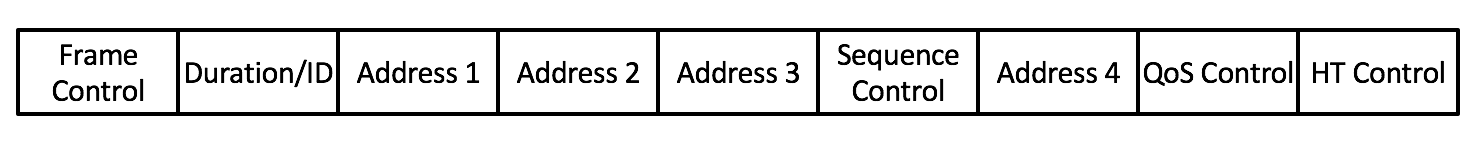
\includegraphics[width=\linewidth]{macHeader}}
			\caption{\ac{MPDU} format when using \ac{WPA}-2 \cite{802.11}}
			\label{fig:MpduFormat}
		\end{center}
		\vspace{-0.2 in}
	\end{figure}
}

\newcommand{\figMacHeader}{
	\begin{figure}[H]
		\begin{center}
			\makebox[\textwidth][c]{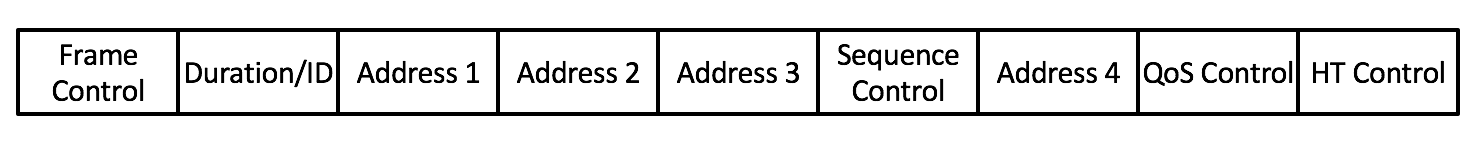
\includegraphics[width=\linewidth]{macHeader}}
			\caption{\ac{MAC} Header Frame Format \cite{802.11}}
			\label{fig:MacHeader}
		\end{center}
		\vspace{-0.2 in}
	\end{figure}
}

\newcommand{\figArchitecture}{\begin{figure}[H]
	\begin{center}
		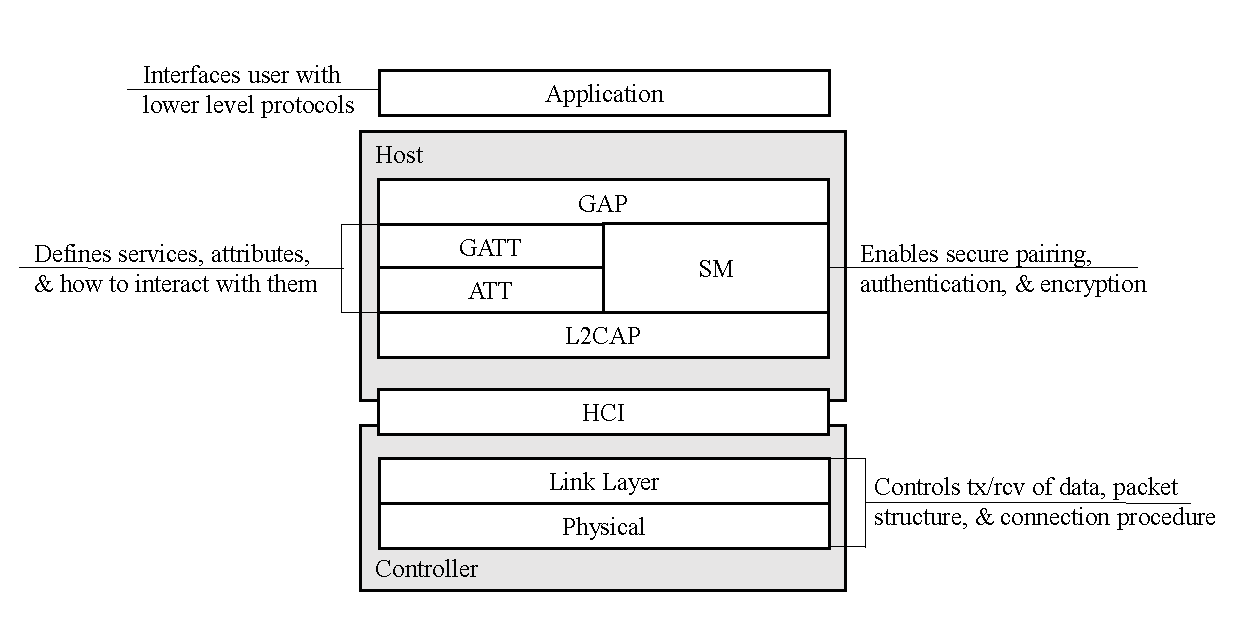
\includegraphics[width=4in]{architecture}
		\caption{The Bluetooth Low Energy Architecture}
		\label{fig:Architecture}
	\end{center}
	\vspace{-0.2 in}
\end{figure}
}

\newcommand{\figConnection}{\begin{figure}[H]
	\begin{center}
		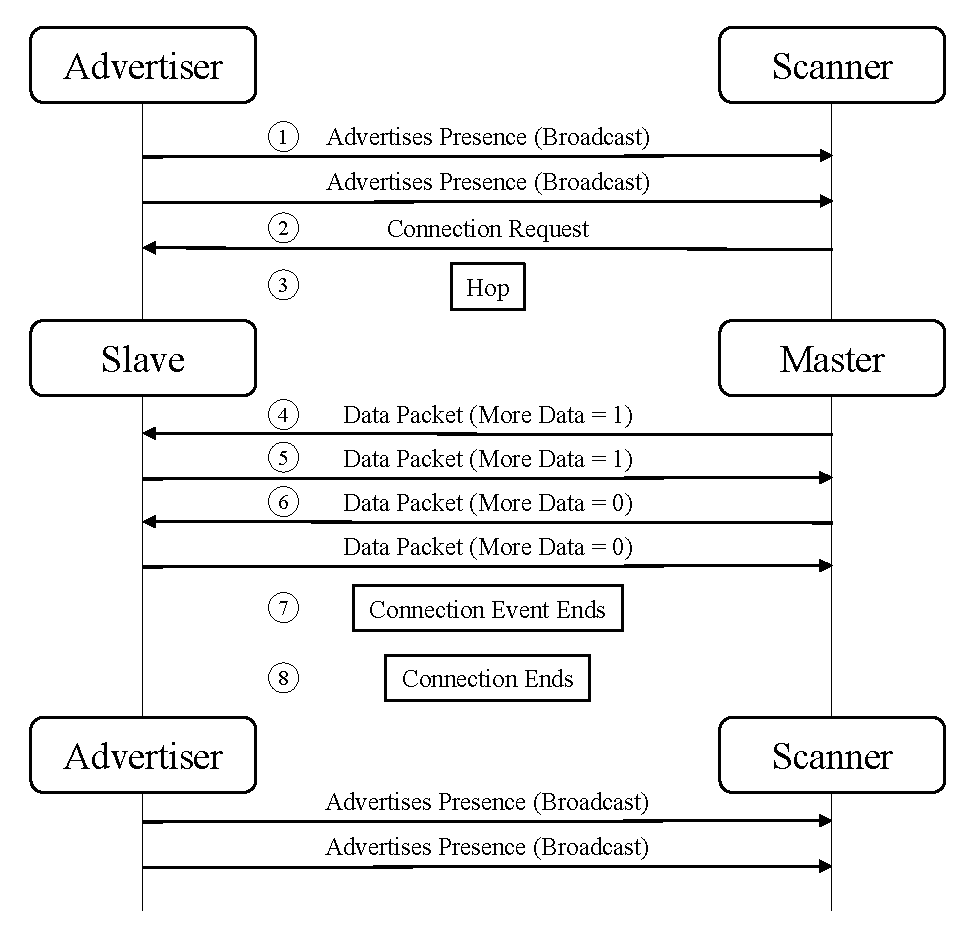
\includegraphics[width=4in]{connectionProcess}
		\caption{The \ac{BLE} Connection Process}
		\label{fig:Connection}
	\end{center}
	\vspace{-0.2 in}
\end{figure}
}

\newcommand{\figScanning}{\begin{figure}[H]
		\begin{center}
			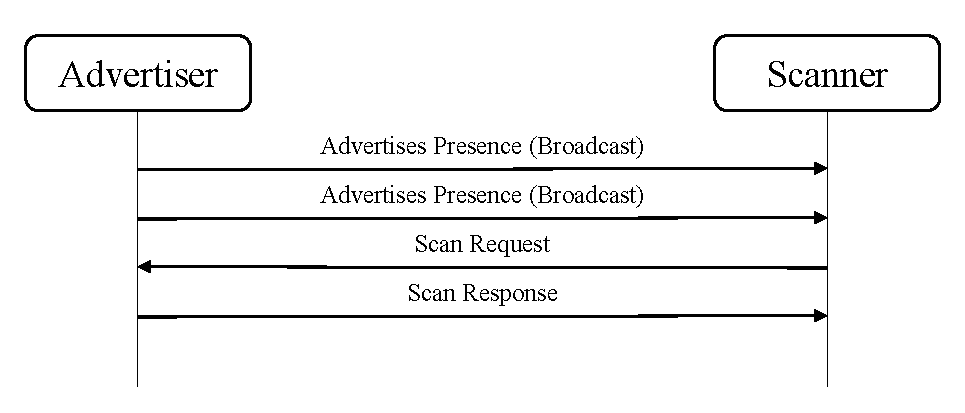
\includegraphics[width=4in]{activeScanning}
			\caption{Active Scanning Process}
			\label{fig:Scanning}
		\end{center}
		\vspace{-0.2 in}
	\end{figure}
}

\newcommand{\figChannel}{
	\begin{figure}[H]
		\begin{center}
			\includegraphics[width=5in]{channelMap}
			\caption{Bluetooth Low Energy channel mapping; darker channels represent advertisement channels}
			\label{fig:Channel}
		\end{center}
		\vspace{-0.2 in}
	\end{figure}
}

\newcommand{\figAccessPoint}{
	\begin{figure}[H]
		\begin{center}
			\makebox[\textwidth][c]{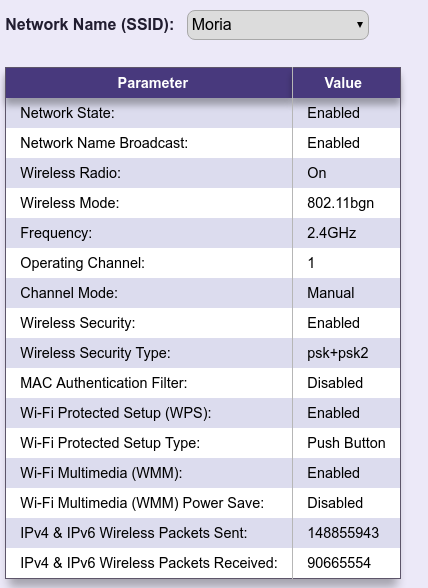
\includegraphics[width=2.5in]{accessPoint}}
			\caption{Prancing Pony Access Point Settings}
			\label{fig:AccessPoint}
		\end{center}
		\vspace{-0.2 in}
	\end{figure}
}

\newcommand{\figSystemDiagram}{
	\begin{figure}[h!]
		\begin{center}
			\centering
			\makebox[\textwidth][c]{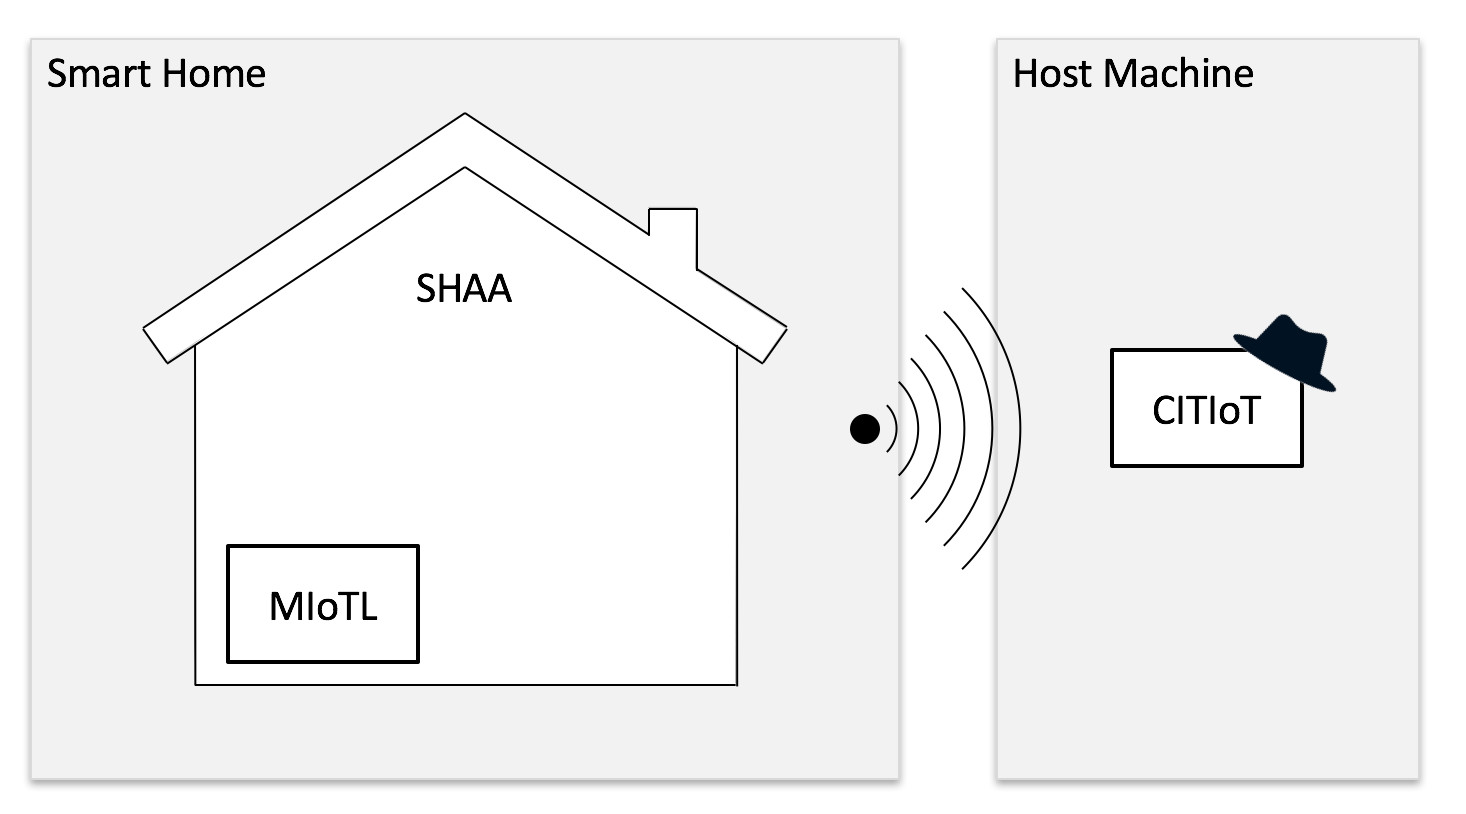
\includegraphics[width=4in]{systemDiagram}}
			\caption{Overall system diagram}
			\label{fig:SystemDiagram}
		\end{center}
		\vspace{-0.2 in}
	\end{figure}
}

\newcommand{\figShaaDiagram}{
	\begin{figure*}[h!]
		\begin{center}
			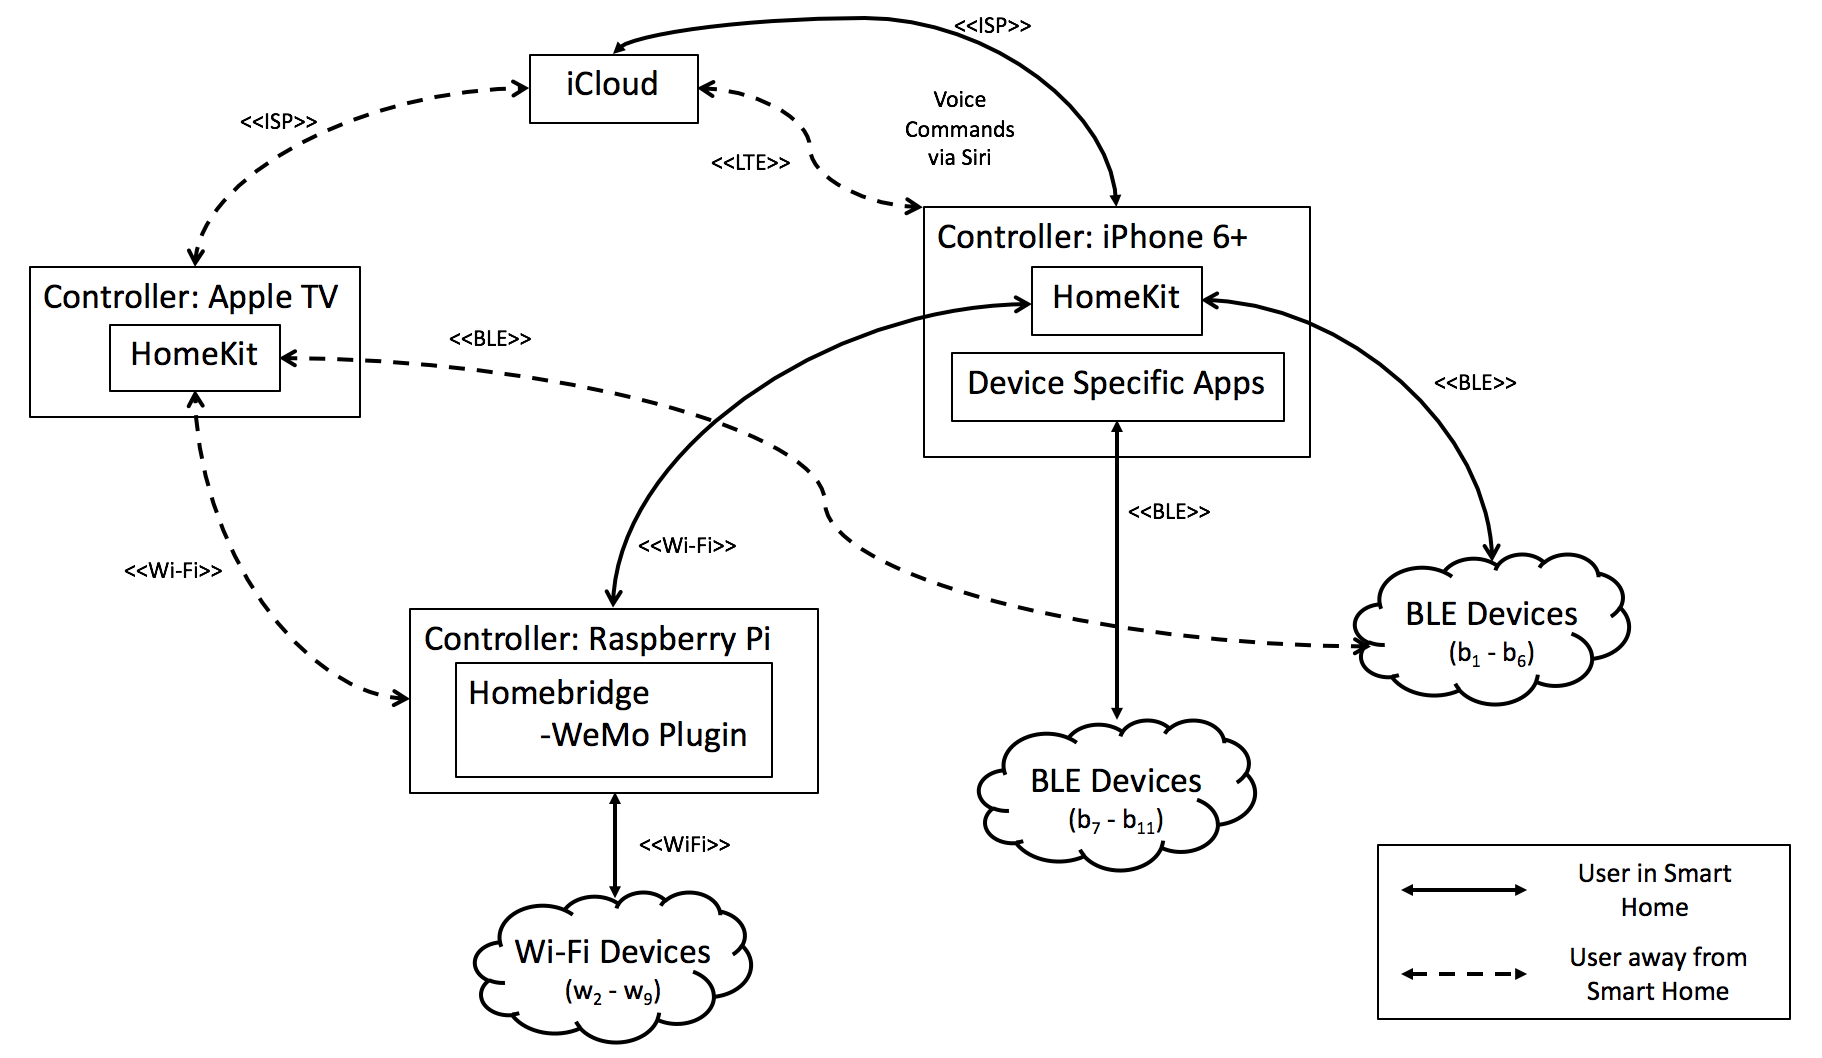
\includegraphics[width=\linewidth]{shaaDiagram}
			\caption{Diagram of SHAA components}
			\label{fig:ShaaDiagram}
		\end{center}
		\vspace{-0.2 in}
	\end{figure*}
}

\newcommand{\figCitiotDiagram}{
	\begin{figure*}[h!]
		\begin{center}
			\makebox[\textwidth][c]{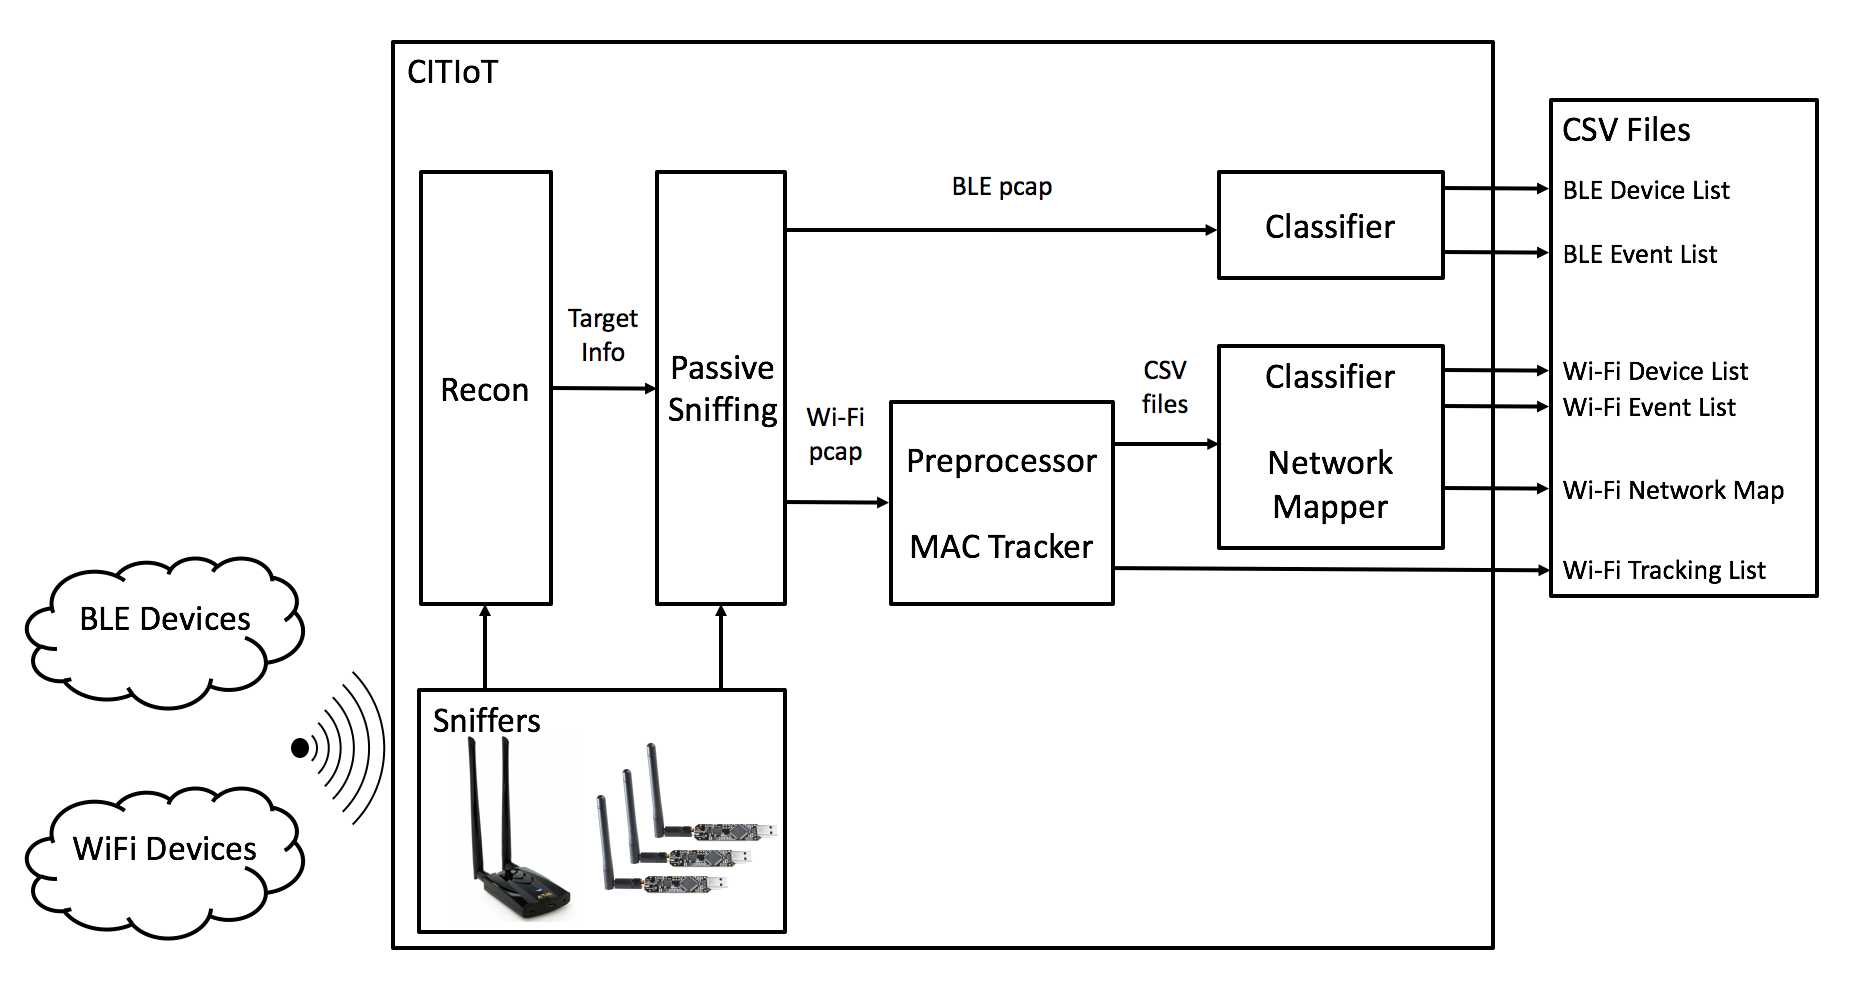
\includegraphics[width=\linewidth]{citiotDiagram}}
			\caption{Diagram of CITIoT tool components and interactions}
			\label{fig:CitiotDiagram}
		\end{center}
		\vspace{-0.2 in}
	\end{figure*}
}

\newcommand{\figReconScan}{
	\begin{figure*}[h!]
		\begin{center}
			\makebox[\textwidth][c]{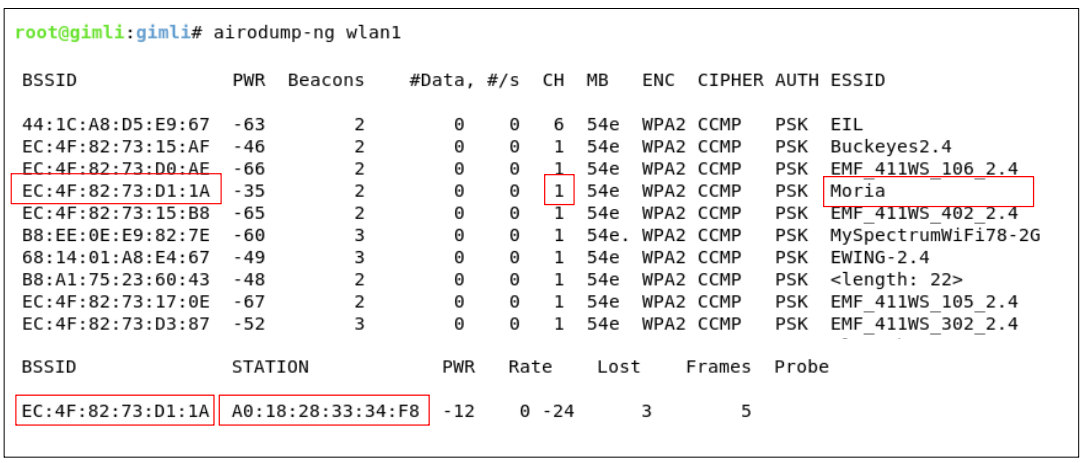
\includegraphics[width=\linewidth]{reconScan}}
			\caption{Command and results to accomplish a scan of Wi-Fi devices and associated \ac{AP}s}
			\label{fig:ReconScan}
		\end{center}
		\vspace{-0.2 in}
	\end{figure*}
}

\newcommand{\figScanDevices}{
	\begin{figure}[H]
		\begin{center}
			\makebox[\textwidth][c]{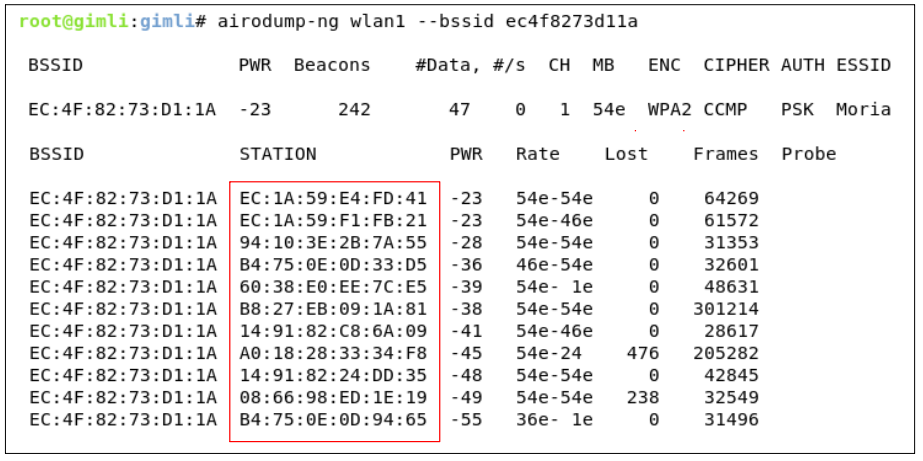
\includegraphics[width=\linewidth]{scanDevices}}
			\caption{Command and results to scan for devices connected to the target \ac{AP}}
			\label{fig:ScanDevices}
		\end{center}
		\vspace{-0.2 in}
	\end{figure}
}

\newcommand{\figOuiLookup}{
	\begin{figure}[H]
		\begin{center}
			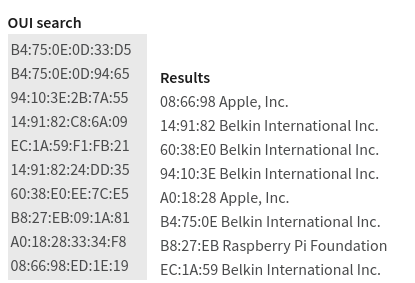
\includegraphics[width=3in]{ouiLookup}
			\caption{Wi-Fi MAC OUI search and results}
			\label{fig:OuiLookup}
		\end{center}
		\vspace{-0.2 in}
	\end{figure}
}

\newcommand{\figBleDeviceScan}{
	\begin{figure}[H]
		\begin{center}
			\makebox[\textwidth][c]{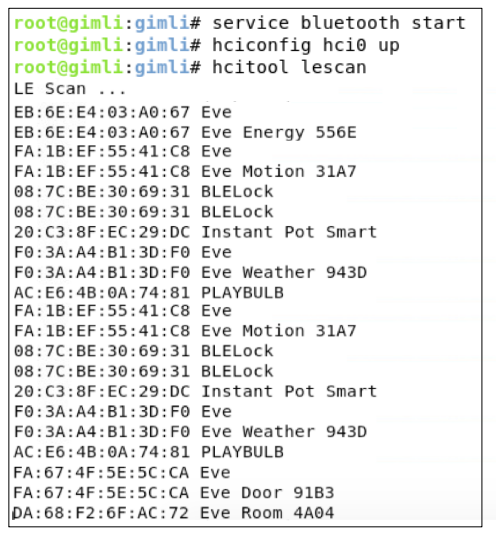
\includegraphics[width=3.5in]{bleDeviceScan}}
			\caption{Command and results to scan for \ac{BLE} devices within the smart home}
			\label{fig:BleDeviceScan}
		\end{center}
		\vspace{-0.2 in}
	\end{figure}
}

\newcommand{\figMonitorMode}{
	\begin{figure}[H]
		\begin{center}
			\makebox[\textwidth][c]{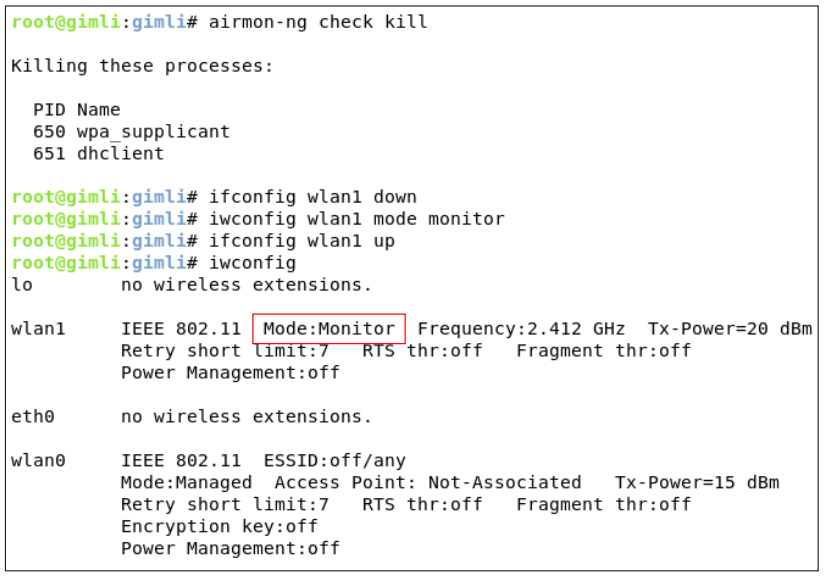
\includegraphics[width=\linewidth]{monitorMode}}
			\caption{Commands used to set Wi-Fi interface to monitor mode}
			\label{fig:MonitorMode}
		\end{center}
		\vspace{-0.2 in}
	\end{figure}
}

\newcommand{\figWifiCaptCmd}{
	\begin{figure}[H]
		\begin{center}
			\makebox[\textwidth][c]{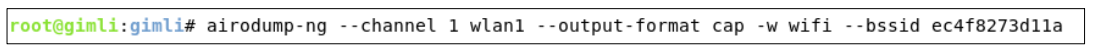
\includegraphics[height=.75cm]{wifiCaptCmd}}
			\caption{Command and options used to capture Wi-Fi traffic}
			\label{fig:WifiCaptCmd}
		\end{center}
		\vspace{-0.2 in}
	\end{figure}
}

\newcommand{\figBleCaptCmd}{
	\begin{figure}[H]
		\begin{center}
			\makebox[\textwidth][c]{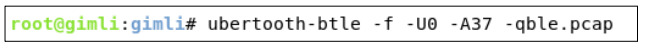
\includegraphics[height=.75cm]{bleCaptCmd}}
			\caption{Example command and options used to capture \ac{BLE} traffic}
			\label{fig:BleCaptCmd}
		\end{center}
		\vspace{-0.2 in}
	\end{figure}
}

\newcommand{\figCorruptTimePacket}{
	\begin{figure}[H]
		\begin{center}
			\makebox[\textwidth][c]{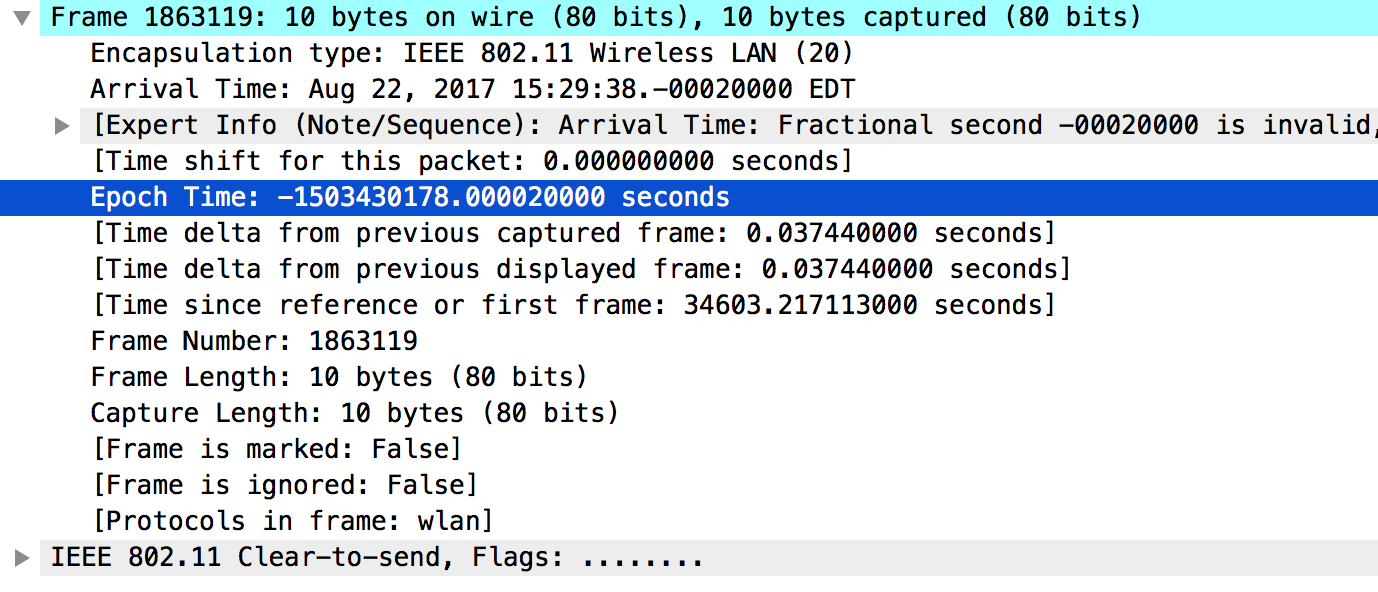
\includegraphics[width=\linewidth]{corruptTimePacket}}
			\caption{Encrypted packet used in \ac{MAC} tracker showing corrupted timestamp}
			\label{fig:CorruptTimePacket}
		\end{center}
		\vspace{-0.2 in}
	\end{figure}
}

\newcommand{\figWrongFrameNumber}{
	\begin{figure}[H]
		\begin{center}
			\makebox[\textwidth][c]{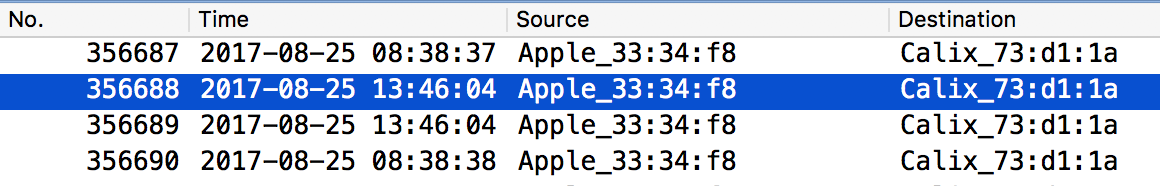
\includegraphics[width=\linewidth]{wrongFrameNumber}}
			\caption{Encrypted packets used in \ac{MAC} tracker showing sequential frame numbers but wrong times}
			\label{fig:WrongFrameNumber}
		\end{center}
		\vspace{-0.2 in}
	\end{figure}
}

\newcommand{\figTrainingToDevice}{
	\begin{figure}[H]
		\centering
		\begin{subfigure}{.485\textwidth}
			\centering
			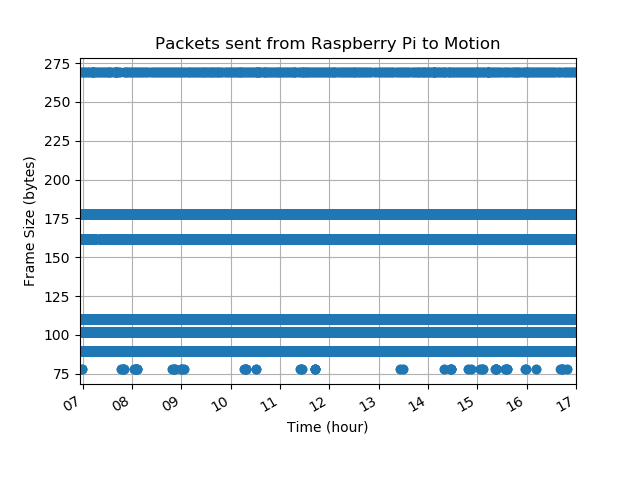
\includegraphics[width=\linewidth]{trngToMotion}
			\caption{}
		\end{subfigure}%
		\begin{subfigure}{.485\textwidth}
			\centering
			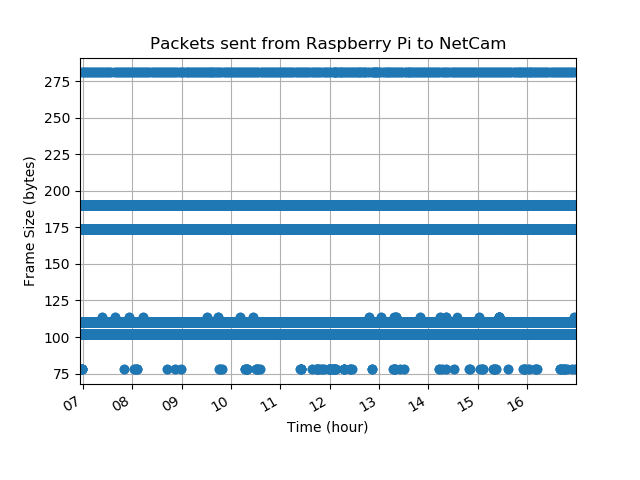
\includegraphics[width=\linewidth]{trngToNetcam}
			\caption{}
		\end{subfigure}
		\begin{subfigure}{.485\textwidth}
			\centering
			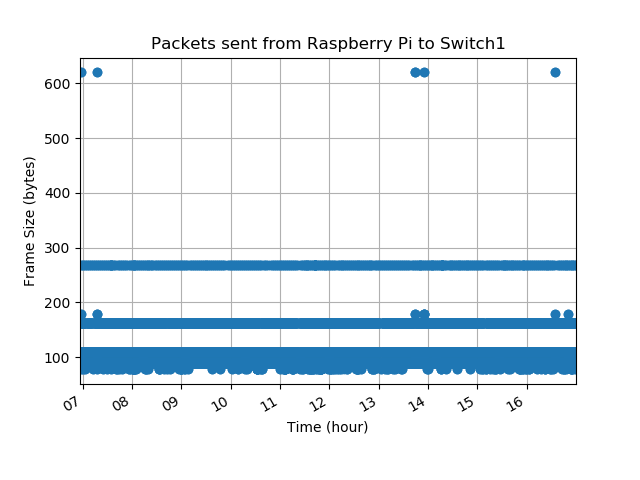
\includegraphics[width=\linewidth]{trngToSwitch1}
			\caption{}
		\end{subfigure}%
		\begin{subfigure}{.485\textwidth}
			\centering
			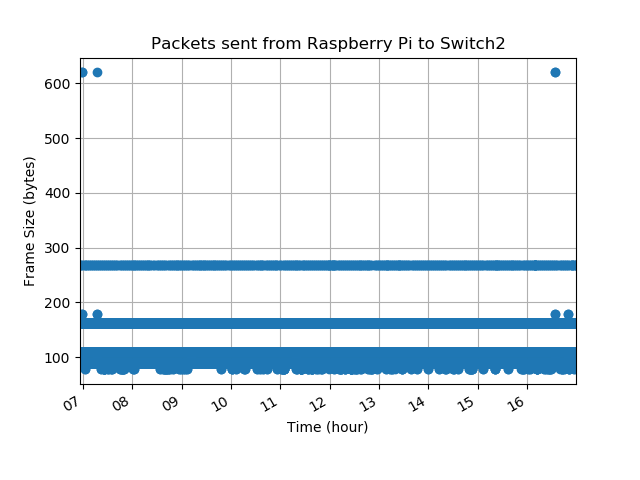
\includegraphics[width=\linewidth]{trngToSwitch2}
			\caption{}
		\end{subfigure}
		\begin{subfigure}{.485\textwidth}
			\centering
			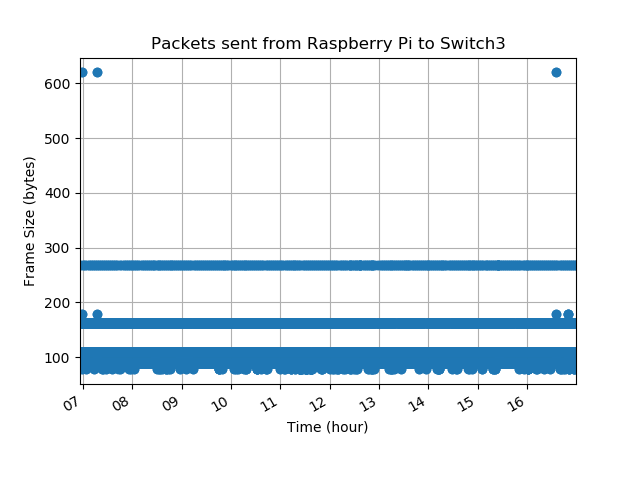
\includegraphics[width=\linewidth]{trngToSwitch3}
			\caption{}
		\end{subfigure}%
		\begin{subfigure}{.485\textwidth}
			\centering
			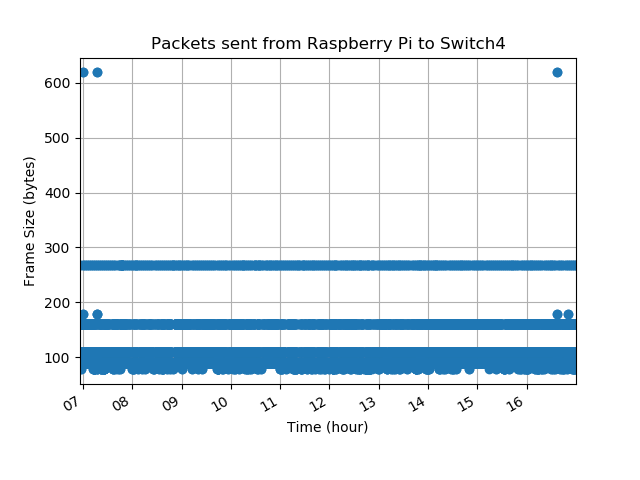
\includegraphics[width=\linewidth]{trngToSwitch4}
			\caption{}
		\end{subfigure}
		\begin{subfigure}{.485\textwidth}
			\centering
			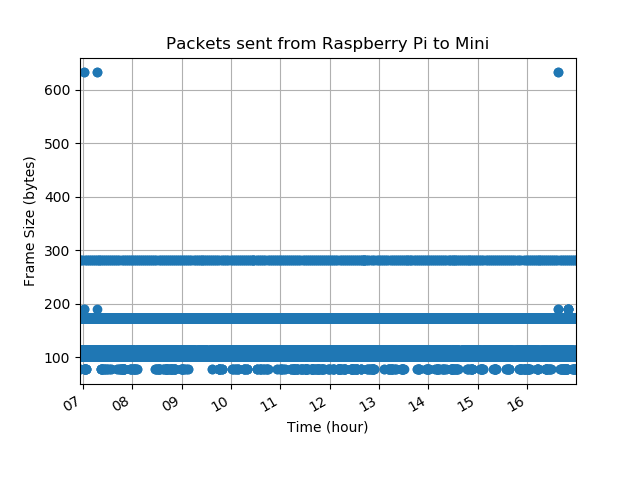
\includegraphics[width=\linewidth]{trngToMini}
			\caption{}
		\end{subfigure}%
		\begin{subfigure}{.485\textwidth}
			\centering
			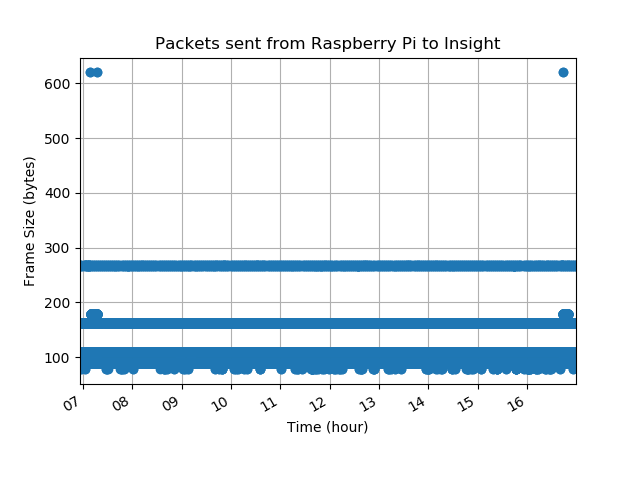
\includegraphics[width=\linewidth]{trngToInsight}
			\caption{}
		\end{subfigure}
		\caption{Training plots of packets sent from raspberry pi to device}
		\label{fig:TrainingToDevice}
	\end{figure}
}

\newcommand{\figTrainingFromDevice}{
	\begin{figure}[H]
		\centering
		\begin{subfigure}{.485\textwidth}
			\centering
			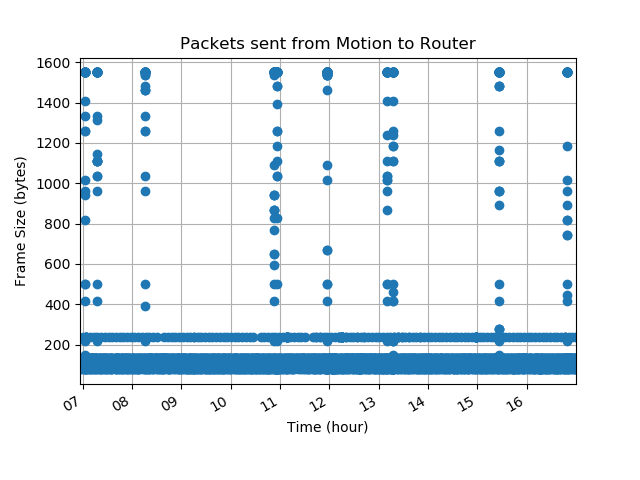
\includegraphics[width=\linewidth]{trngFromMotion}
			\caption{}
		\end{subfigure}%
		\begin{subfigure}{.485\textwidth}
			\centering
			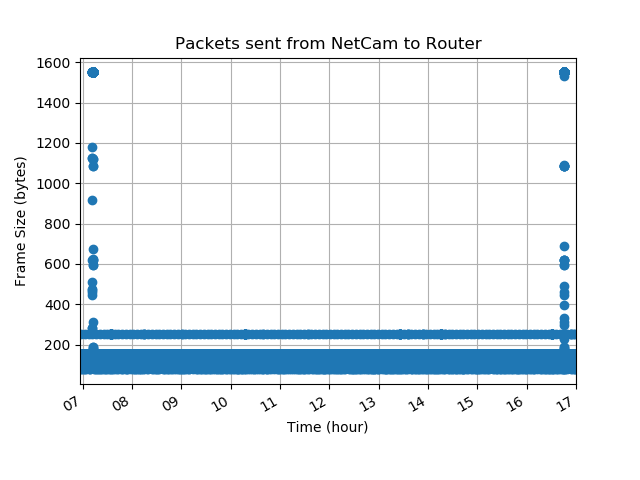
\includegraphics[width=\linewidth]{trngFromNetcam}
			\caption{}
		\end{subfigure}
		\begin{subfigure}{.485\textwidth}
			\centering
			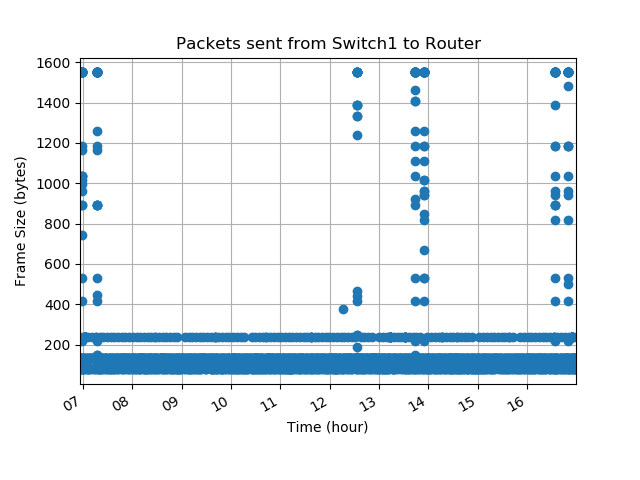
\includegraphics[width=\linewidth]{trngFromSwitch1}
			\caption{}
		\end{subfigure}%
		\begin{subfigure}{.485\textwidth}
			\centering
			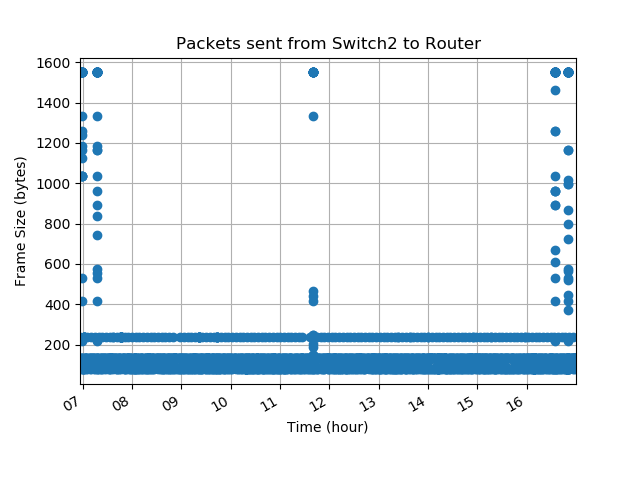
\includegraphics[width=\linewidth]{trngFromSwitch2}
			\caption{}
		\end{subfigure}
		\begin{subfigure}{.485\textwidth}
			\centering
			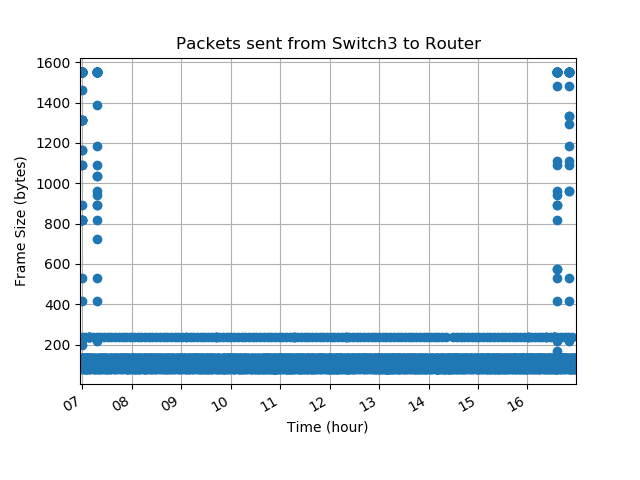
\includegraphics[width=\linewidth]{trngFromSwitch3}
			\caption{}
		\end{subfigure}%
		\begin{subfigure}{.485\textwidth}
			\centering
			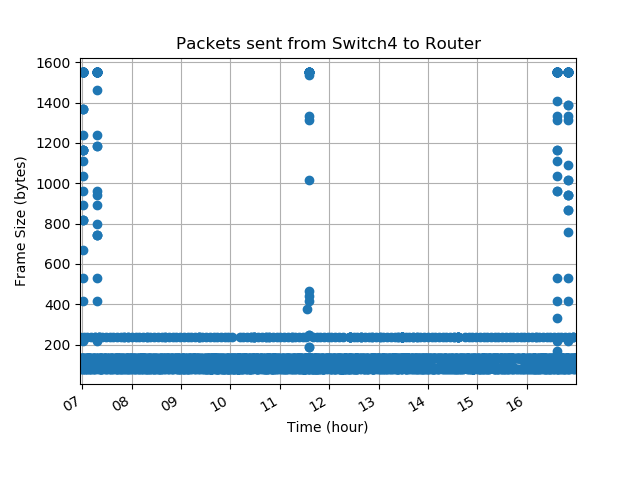
\includegraphics[width=\linewidth]{trngFromSwitch4}
			\caption{}
		\end{subfigure}
		\begin{subfigure}{.485\textwidth}
			\centering
			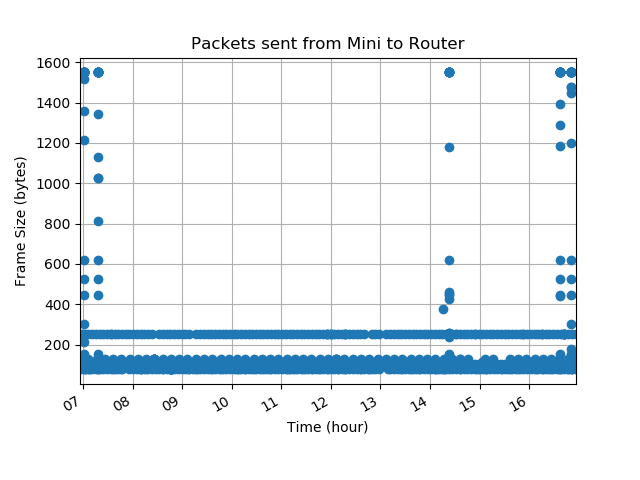
\includegraphics[width=\linewidth]{trngFromMini}
			\caption{}
		\end{subfigure}%
		\begin{subfigure}{.485\textwidth}
			\centering
			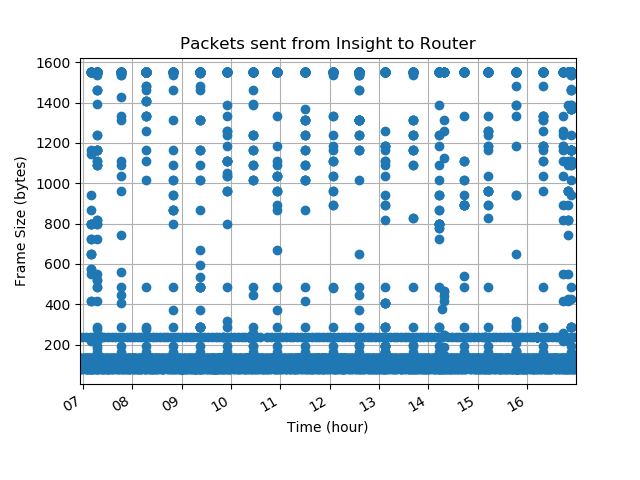
\includegraphics[width=\linewidth]{trngFromInsight}
			\caption{}
		\end{subfigure}
		\caption{Training plots of packets sent from device to the router}
		\label{fig:TrainingFromDevice}
	\end{figure}
}

\newcommand{\figClassificationToNetcam}{
	\begin{figure}[H]
		\begin{center}
			\makebox[\textwidth][c]{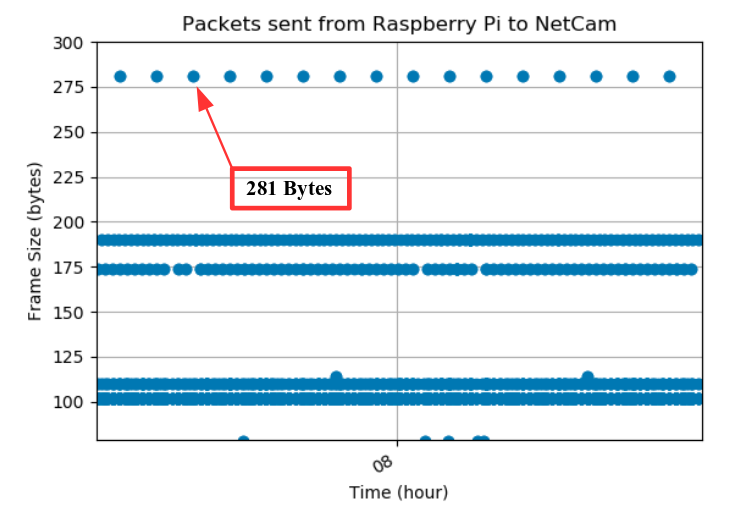
\includegraphics[width=5in]{classificationToNetcam}}
			\caption{Figure~\ref{fig:TrainingToDevice}(b) zoomed in on unique packet traffic used to classify camera devices}
			\label{fig:ClassificationToNetcam}
		\end{center}
		\vspace{-0.2 in}
	\end{figure}
}

\newcommand{\figClassificationToMotion}{
	\begin{figure}[H]
		\begin{center}
			\makebox[\textwidth][c]{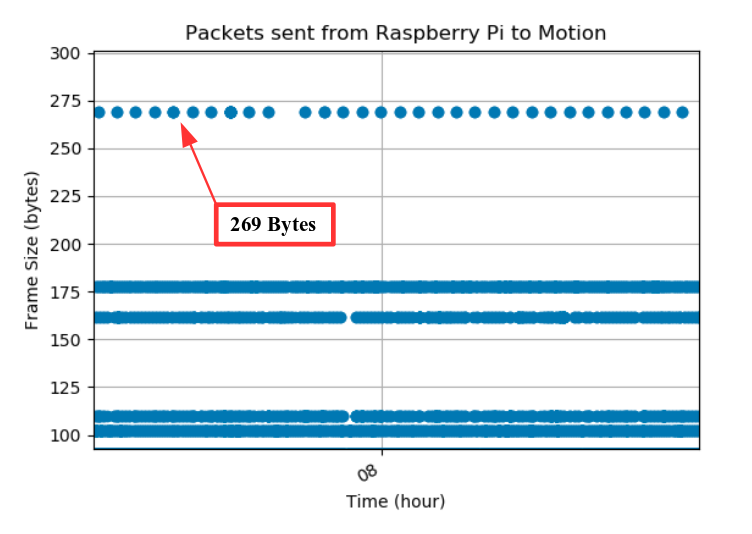
\includegraphics[width=5in]{classificationToMotion}}
			\caption{Figure~\ref{fig:TrainingToDevice}(a) zoomed in on unique packet traffic used to classify motion devices}
			\label{fig:ClassificationToMotion}
		\end{center}
		\vspace{-0.2 in}
	\end{figure}
}

\newcommand{\figClassificationToSwitch}{
	\begin{figure}[H]
		\begin{center}
			\makebox[\textwidth][c]{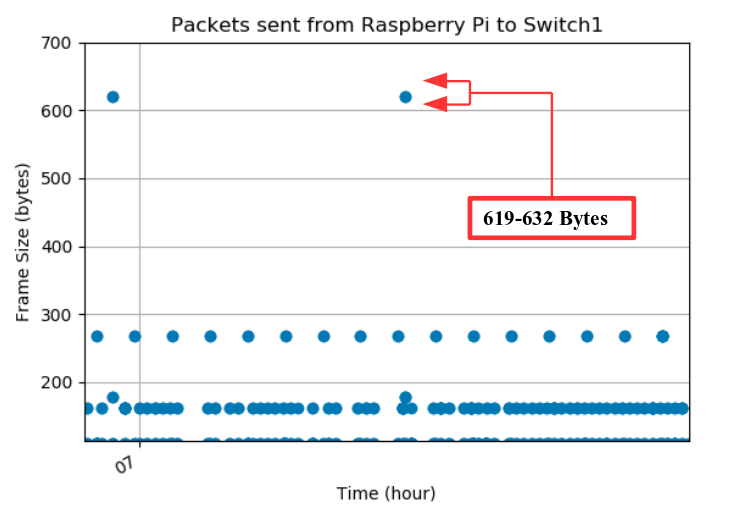
\includegraphics[width=5in]{classificationToSwitch}}
			\caption{Figure~\ref{fig:TrainingToDevice}(c) zoomed in on unique packet traffic used to classify outlet devices}
			\label{fig:ClassificationToSwitch}
		\end{center}
		\vspace{-0.2 in}
	\end{figure}
}

\newcommand{\figDeviceClassification}{
	\begin{figure}[H]
		\begin{center}
			\makebox[\textwidth][c]{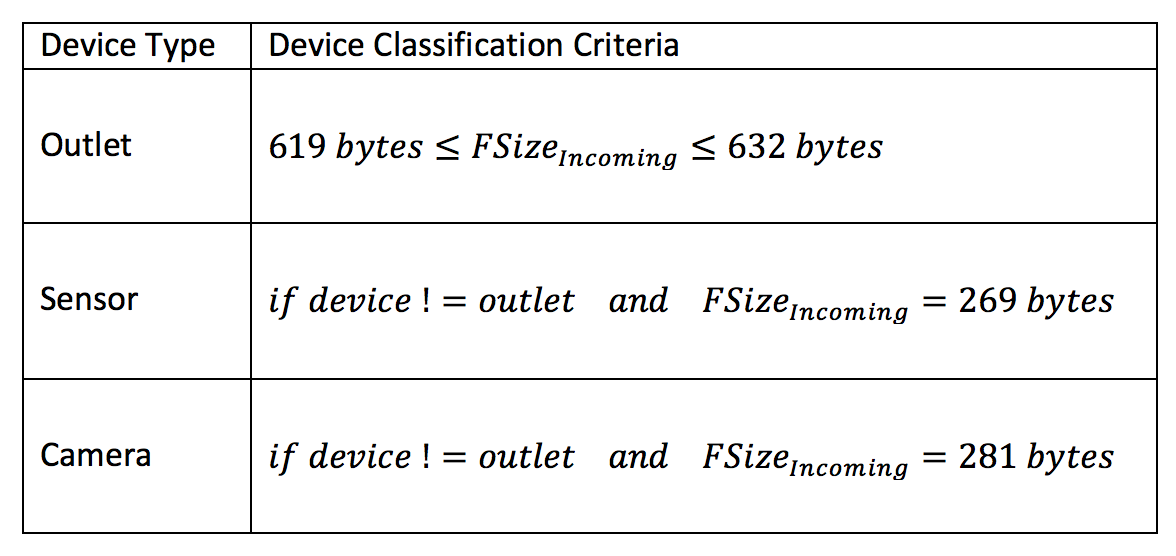
\includegraphics[height=2in]{deviceClassification}}
			\caption{Criteria used to classify devices}
			\label{fig:DeviceClassification}
		\end{center}
		\vspace{-0.2 in}
	\end{figure}
}

\newcommand{\figIdentificationToMini}{
	\begin{figure}[H]
		\begin{center}
			\makebox[\textwidth][c]{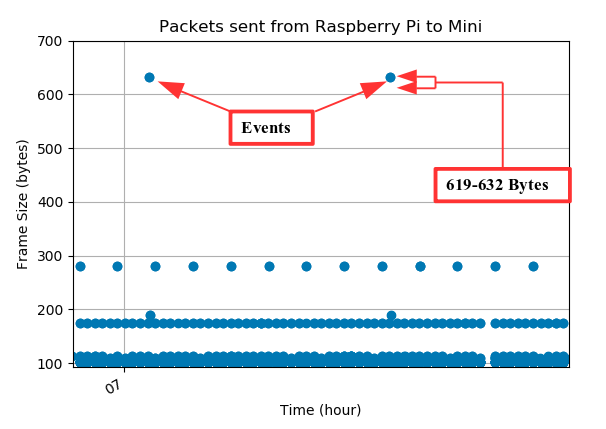
\includegraphics[width=5in]{identificationToMini}}
			\caption{Figure~\ref{fig:TrainingToDevice}(g) zoomed in on unique packet traffic used to identify outlet events}
			\label{fig:IdentificationToMini}
		\end{center}
		\vspace{-0.2 in}
	\end{figure}
}

\newcommand{\figIdentificationFromNetcam}{
	\begin{figure}[H]
		\begin{center}
			\makebox[\textwidth][c]{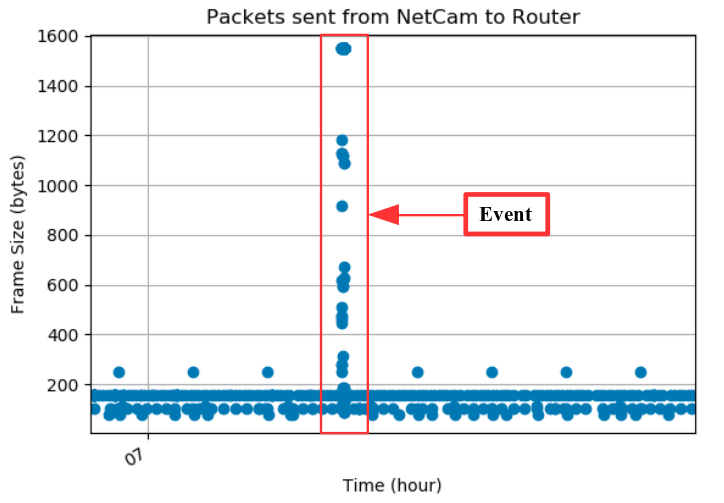
\includegraphics[width=5in]{identificationFromNetcam}}
			\caption{Figure~\ref{fig:TrainingFromDevice}(b) zoomed in on unique packet traffic used to identify camera events}
			\label{fig:IdentificationFromNetcam}
		\end{center}
		\vspace{-0.2 in}
	\end{figure}
}

\newcommand{\figIdentificationFromNetcamCum}{
	\begin{figure}[H]
		\begin{center}
			\makebox[\textwidth][c]{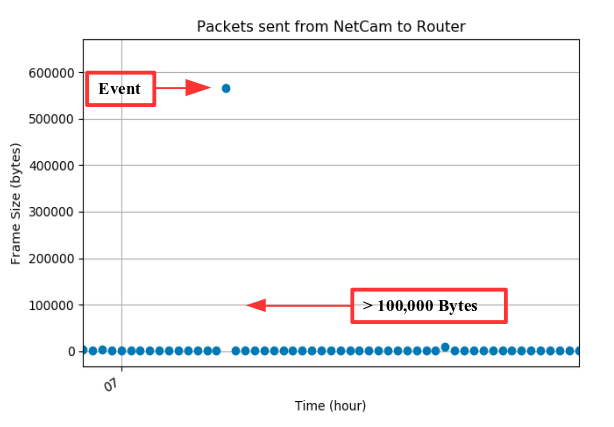
\includegraphics[width=5in]{identificationFromNetcamCum}}
			\caption{Figure~\ref{fig:TrainingFromDevice}(b) with one minute cumulative frame size zoomed in on unique packet traffic used to identify camera events}
			\label{fig:IdentificationFromNetcamCum}
		\end{center}
		\vspace{-0.2 in}
	\end{figure}
}

\newcommand{\figIdentificationFromMotion}{
	\begin{figure}[H]
		\begin{center}
			\makebox[\textwidth][c]{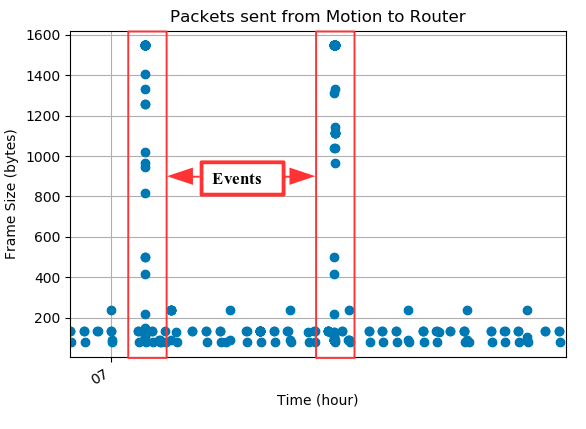
\includegraphics[width=5in]{identificationFromMotion}}
			\caption{Figure~\ref{fig:TrainingFromDevice}(a) zoomed in on unique packet traffic used to identify motion events}
			\label{fig:IdentificationFromMotion}
		\end{center}
		\vspace{-0.2 in}
	\end{figure}
}

\newcommand{\figIdentificationFromMotionCum}{
	\begin{figure}[H]
		\begin{center}
			\makebox[\textwidth][c]{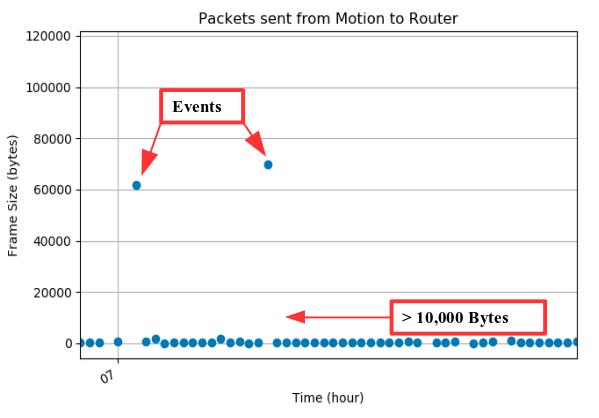
\includegraphics[width=5in]{identificationFromMotionCum}}
			\caption{Figure~\ref{fig:TrainingFromDevice}(a) with one minute cumulative frame size zoomed in on unique packet traffic used to identify motion events}
			\label{fig:IdentificationFromMotionCum}
		\end{center}
		\vspace{-0.2 in}
	\end{figure}
}

\newcommand{\figEventIdentification}{
	\begin{figure}[H]
		\begin{center}
			\makebox[\textwidth][c]{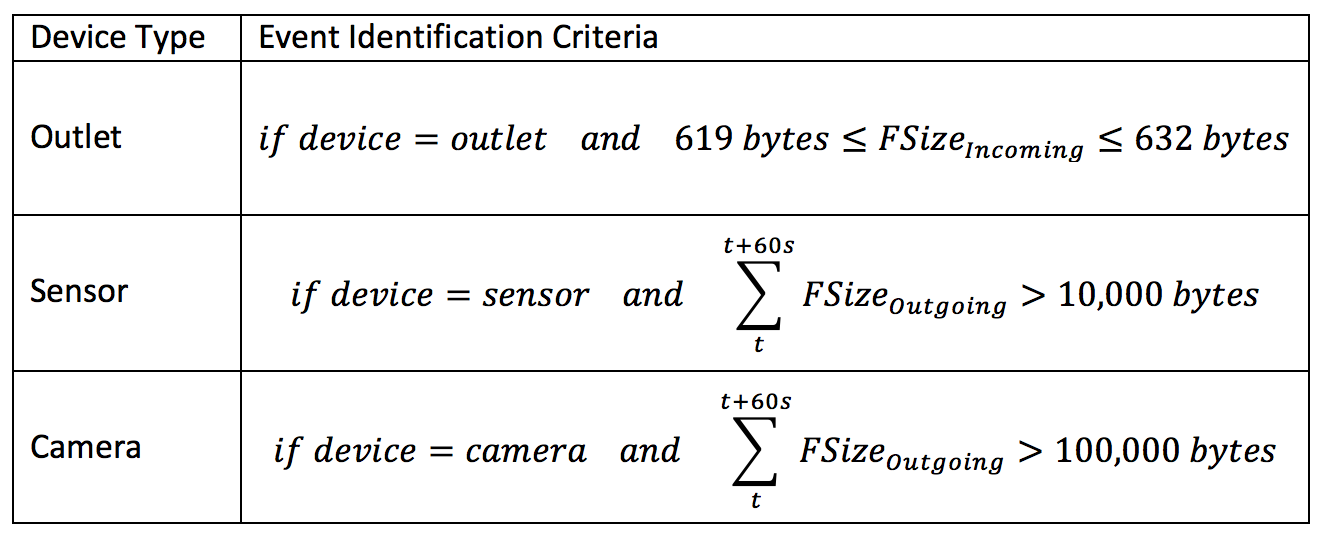
\includegraphics[height=2in]{eventIdentification}}
			\caption{Criteria used to identify events}
			\label{fig:EventIdentification}
		\end{center}
		\vspace{-0.2 in}
	\end{figure}
}

\newcommand{\figSubscribePacket}{
	\begin{figure}[H]
		\begin{center}
			\makebox[\textwidth][c]{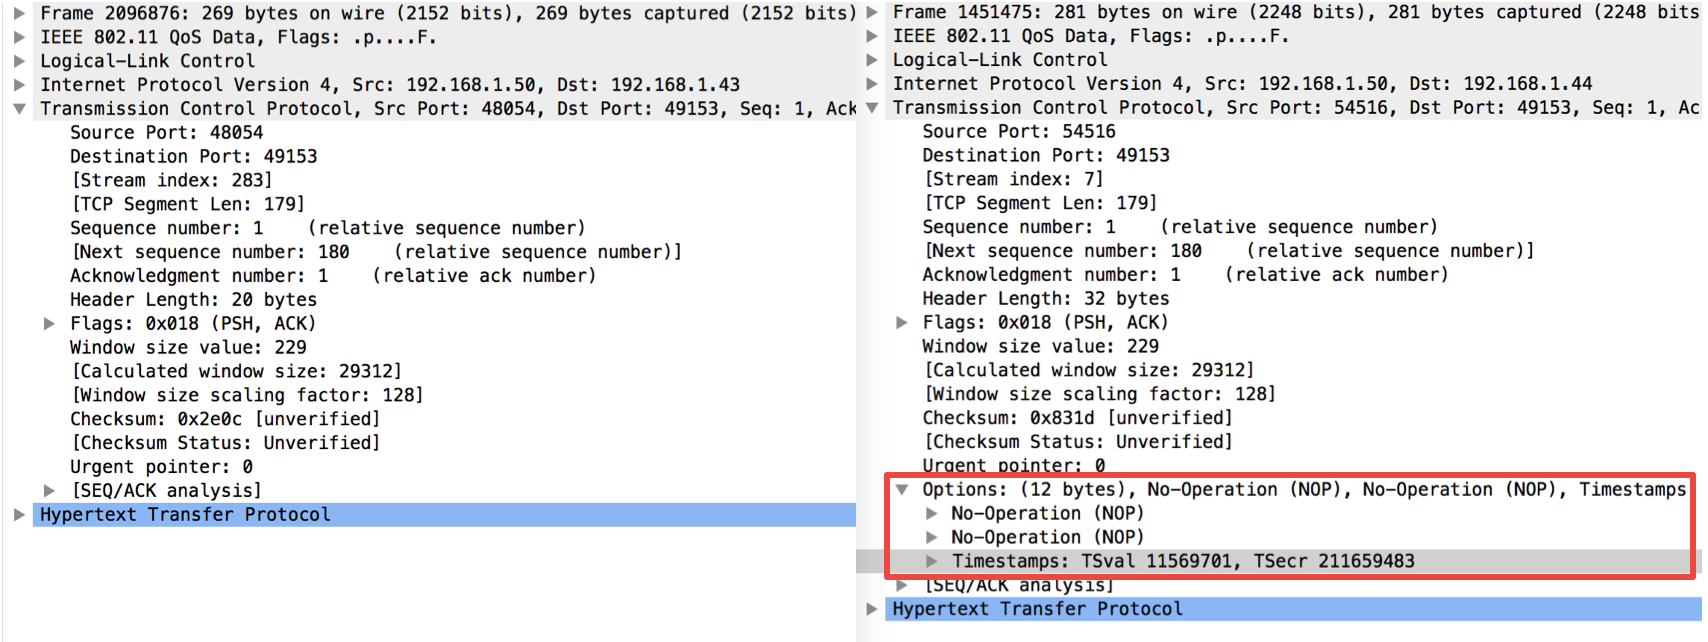
\includegraphics[width=\linewidth]{subscribePacket}}
			\caption{Decrypted \texttt{SUBSCRIBE} packets from Raspberry Pi to the NetCam and Motion devices depicting difference in frame length}
			\label{fig:SubscribePacket}
		\end{center}
		\vspace{-0.2 in}
	\end{figure}
}

\newcommand{\figPostPacket}{
	\begin{figure}[H]
		\begin{center}
			\makebox[\textwidth][c]{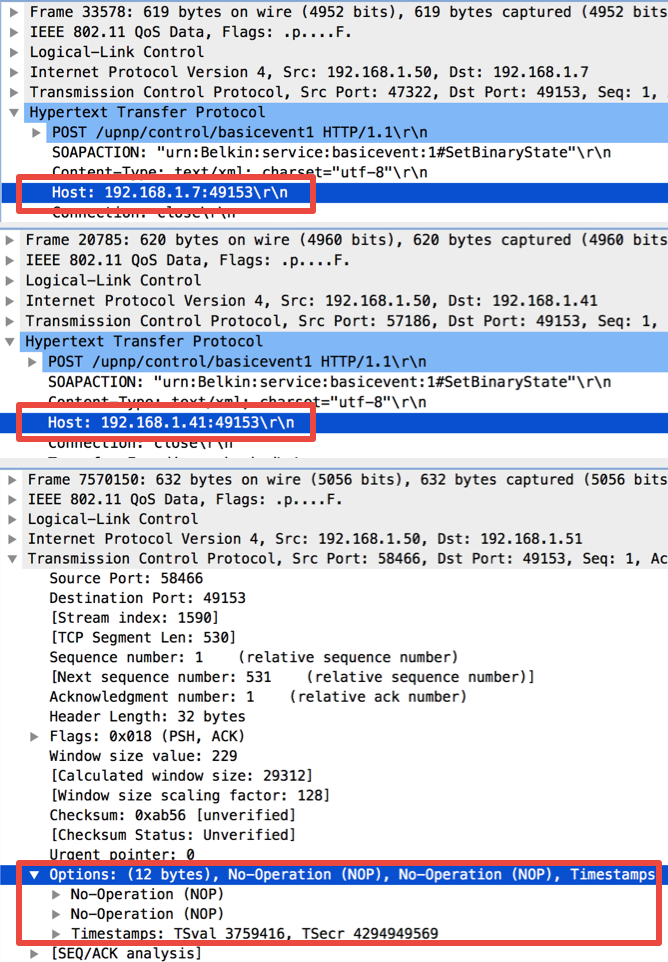
\includegraphics[width=.975\linewidth]{postPacket}}
			\caption{Decrypted \texttt{POST} packets from Raspberry Pi to the Switch4, Switch2, and Mini depicting differences in frame length}
			\label{fig:PostPacket}
		\end{center}
		\vspace{-0.2 in}
	\end{figure}
}

\newcommand{\figNetworkMap}{
	\begin{figure}[H]
		\begin{center}
			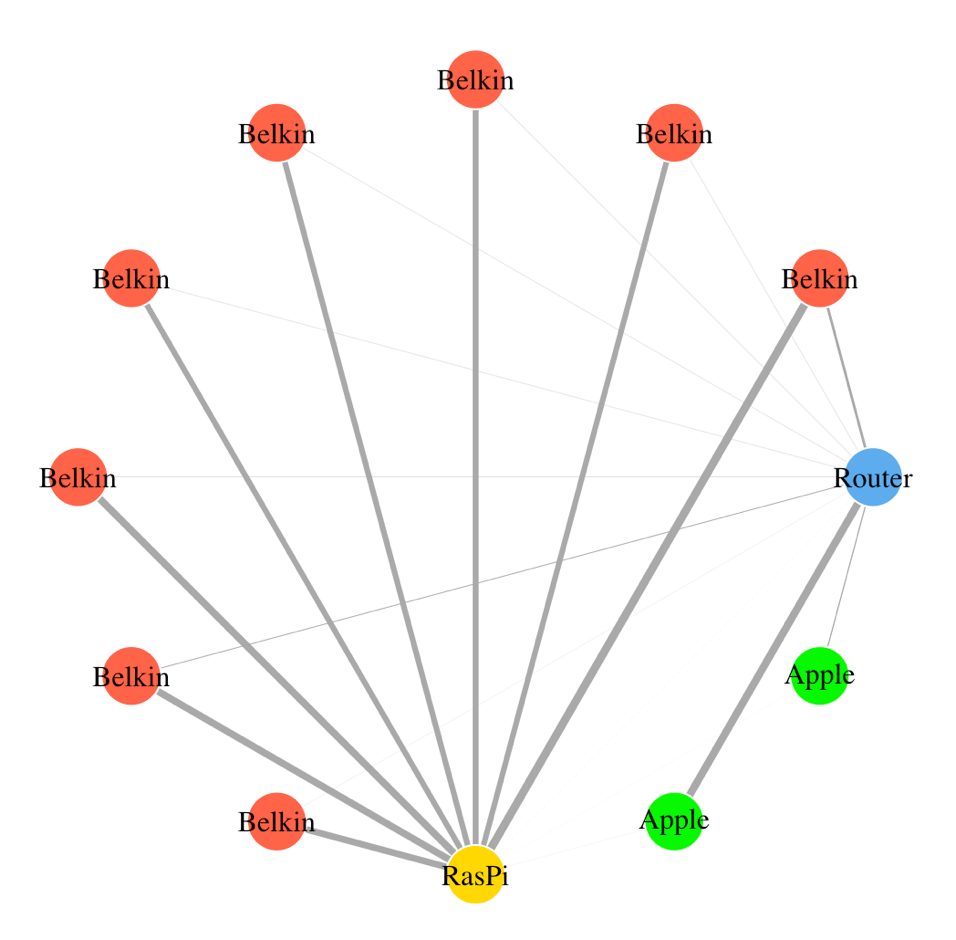
\includegraphics[width=5in]{networkMap}
			\caption{Network mapping of smart home architecture}
			\label{fig:NetworkMap}
		\end{center}
		\vspace{-0.2 in}
	\end{figure}
}

\newcommand{\figMiotlDiagram}{
	\begin{figure*}[h!]
		\begin{center}
			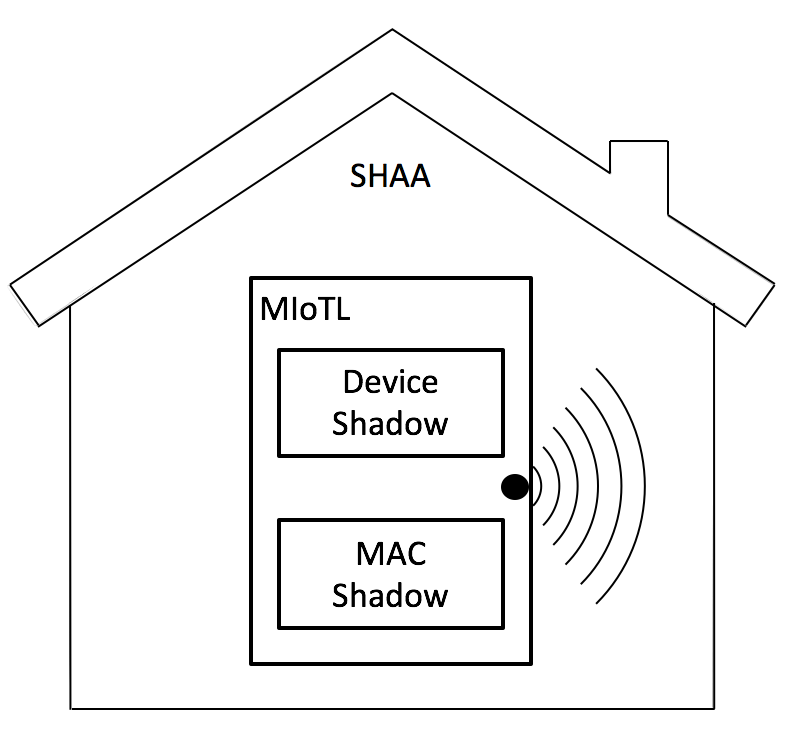
\includegraphics[width=3in]{miotlDiagram}
			\caption{Diagram of MIoTL tool components}
			\label{fig:MiotlDiagram}
		\end{center}
		\vspace{-0.2 in}
	\end{figure*}
}

\newcommand{\figSutCutDiagram}{
	\begin{figure*}[h!]
		\begin{center}
			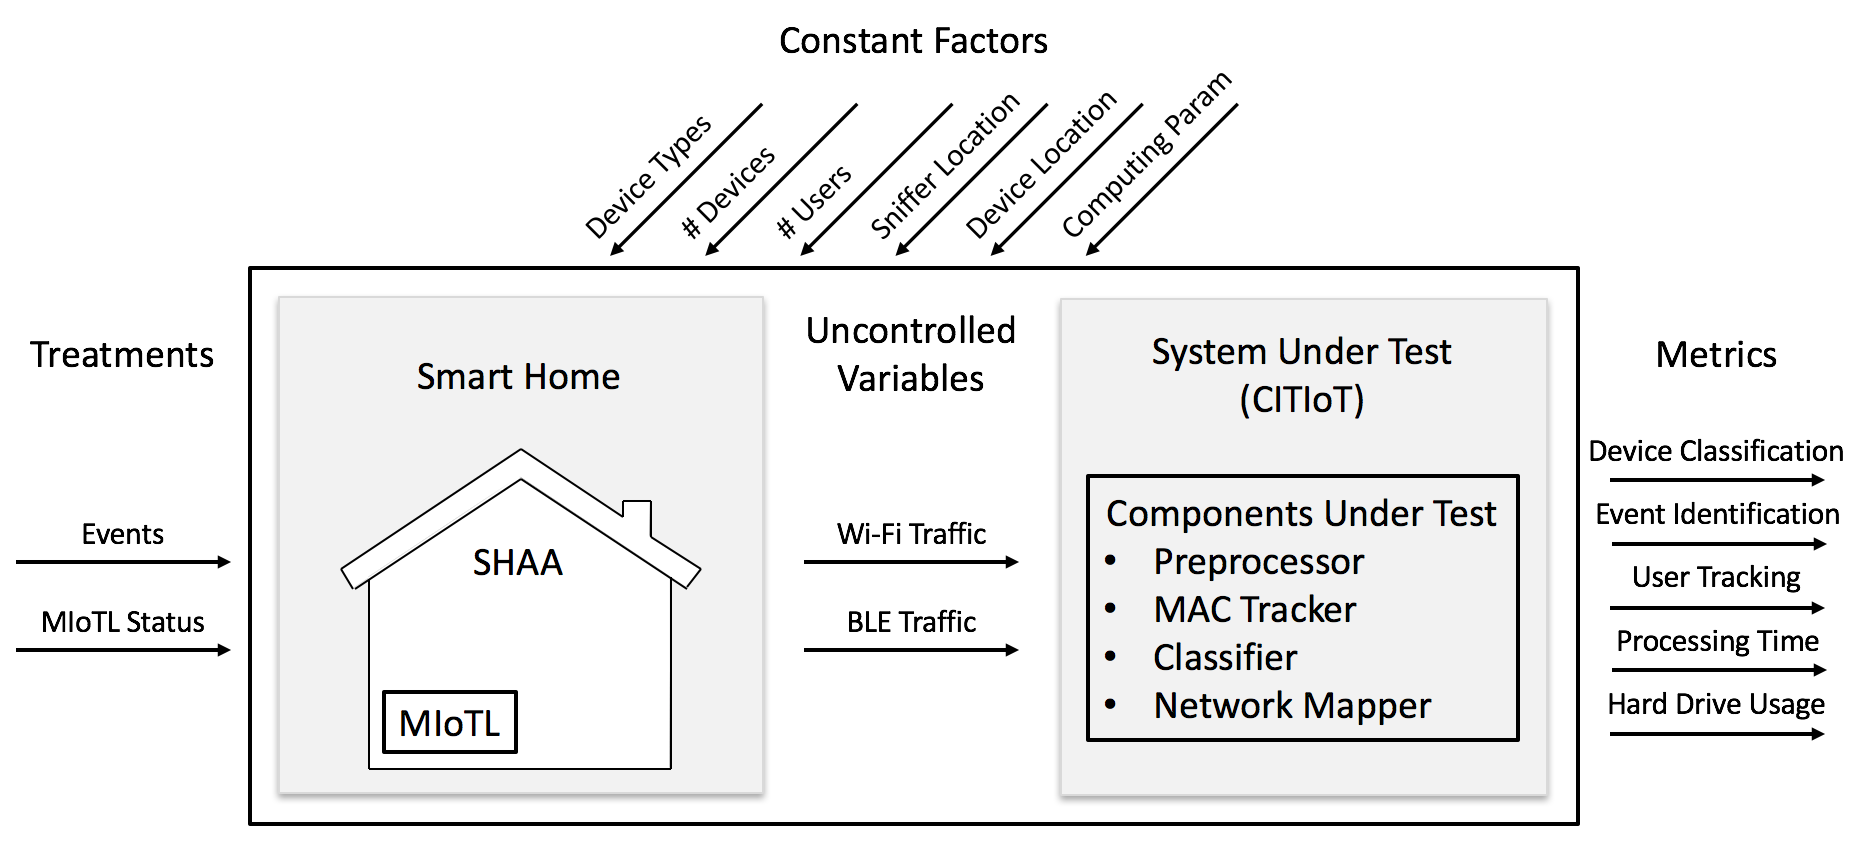
\includegraphics[width=\linewidth]{sutCutDiagram}
			\caption{System Under Test (SUT) and Component Under Test (CUT) diagram}
			\label{fig:SutCutDiagram}
		\end{center}
		\vspace{-0.2 in}
	\end{figure*}
}

\newcommand{\figShaaExperimentDiagram}{
	\begin{figure*}[h!]
		\begin{center}
			\includegraphics[width=\linewidth]{shaaExperimentDiagram}
			\caption{Approximate layout of devices within \ac{SHAA} for experimentation (not to scale)}
			\label{fig:ShaaExperimentDiagram}
		\end{center}
		\vspace{-0.2 in}
	\end{figure*}
}

\newcommand{\figSnifferExperimentSetup}{
	\begin{figure*}[h!]
		\begin{center}
			\includegraphics[width=\linewidth]{snifferExperimentSetup}
			\caption{Layout of sniffer antennae for experimentation}
			\label{fig:SnifferExperimentSetup}
		\end{center}
		\vspace{-0.2 in}
	\end{figure*}
}

\newcommand{\figDataCollectionFramework}{
	\begin{figure}[h!]
		\begin{center}
			\includegraphics[width=\linewidth, height = 5cm]{hostMachine}
			\caption{Data Collection Framework}
			\label{fig:DataCollectionFramework}
		\end{center}
		\vspace{-0.2 in}
	\end{figure}
}

\newcommand{\figSampleResults}{
\begin{figure}[H]
	\begin{center}
		\includegraphics[width=\linewidth]{sampleResults}
		\caption{Example graph comparing CITIoT events with actual events}
		\label{fig:SampleResults}
	\end{center}
	\vspace{-0.2 in}
\end{figure}
}

\newcommand{\figCitiot}{
	\begin{figure}[H]
		\begin{center}
			\makebox[\textwidth][c]{\includegraphics[width=5in]{citiot}}
			\caption{CITIoT Architecture}
			\label{fig:Citiot}
		\end{center}
		\vspace{-0.2 in}
	\end{figure}
}

\newcommand{\figReconScanning}{
	\begin{figure}[H]
		\begin{center}
			\makebox[\textwidth][c]{\includegraphics[width=5in]{reconScanning}}
			\caption{Scanning command along with output.}
			\label{fig:ReconScanning}
		\end{center}
		\vspace{-0.2 in}
	\end{figure}
}

\newcommand{\figNetworkMapping}{
	\begin{figure}[tbp]
		\begin{center}
			\includegraphics[width=3in, height=7cm]{networkMapping}
			\caption{Network mapping of smart home architecture; thicker lines mean stronger correlation between devices.}
			\label{fig:NetworkMapping}
		\end{center}
		\vspace{-0.2 in}
	\end{figure}
}

\newcommand{\figMethodologyOverview}{
	\begin{figure}[H]
		\begin{center}
			\makebox[\textwidth][c]{\includegraphics[width=6in]{methodologyOverview}}
			\caption{Overall scenario setup.}
			\label{fig:MethodologyOverview}
		\end{center}
		\vspace{-0.2 in}
	\end{figure}
}

\newcommand{\figDeviceId}{
	\begin{figure}[H]
	\centering
		\begin{minipage}{.5\textwidth}
			\centering
			\includegraphics[width=1\linewidth]{deviceIdOutlet}
			\caption{Outlet device.}
			\label{fig:DeviceIdOutlet}
		\end{minipage}%
		\begin{minipage}{.5\textwidth}
			\centering
			\includegraphics[width=1\linewidth]{deviceIdSensor}
			\caption{Sensor device.}
			\label{fig:DeviceIdSensor}
		\end{minipage}
		\begin{minipage}{.5\textwidth}
			\centering
			\includegraphics[width=1\linewidth]{deviceIdCamera}
			\caption{Camera device.}
			\label{fig:DeviceIdCamera}
		\end{minipage}
	\end{figure}
}


\newcommand{\figExamplePlotOne}{
	\begin{figure}[H]
		\begin{center}
			\makebox[\textwidth][c]{\includegraphics[width=4.5in]{examplePlot1}}
			\caption{Example Plot One: Event Identification}
			\label{fig:ExamplePlotOne}
		\end{center}
		\vspace{-0.2 in}
	\end{figure}
}

\newcommand{\figExamplePlotTwo}{
	\begin{figure}[H]
		\begin{center}
			\makebox[\textwidth][c]{\includegraphics[width=4.5in]{examplePlot2}}
			\caption{Example Plot Two: Time User is Home}
			\label{fig:ExamplePlotTwo}
		\end{center}
		\vspace{-0.2 in}
		\end{figure}
}

\newcommand{\figafitStyle}{\begin{figure}[tbp]
 \begin{center}
    \includegraphics[width=6in]{myFirstLaTeXafit}
     \caption{Recompile using afitThesis.sty, the AFIT
     thesis style file.}
     \label{fig:afitStyle}
 \end{center}
\end{figure}
}


\newcommand{\figtitlePage}{\begin{figure}[tbp]
 \begin{center}
    \includegraphics[width=6in]{titlePage}
     \caption{Enter student data in titlePage.tex to customize the
     document's first pages.}
     \label{fig:titlePage}
 \end{center}
\end{figure}
}

\newcommand{\figmyFlypage}{\begin{figure}[tbp]
 \begin{center}
    \includegraphics[width=6in]{myFlypage}
     \caption{Here we have compiled the first four page of a thesis.}
     \label{fig:myFlypage}
 \end{center}
\end{figure}
}

\newcommand{\figmyFirstAbstract}{\begin{figure}[tbp]
 \begin{center}
    \includegraphics[width=6in]{myFirstAbstract}
     \caption{Add an abstract to the front matter of your thesis.}
     \label{fig:myFirstAbstract}
 \end{center}
\end{figure}
}

\newcommand{\figmyFigures}{\begin{figure}[tbp]
 \begin{center}
    \includegraphics[width=5in]{myFigures}
     \caption{Consider defining all your figures in one file.}
     \label{fig:myFigures}
 \end{center}
\end{figure}
}


\newcommand{\figmyFirstFigures}{\begin{figure}[tbp]
 \begin{center}
    \includegraphics[width=6in]{myFirstFigures}
     \caption{Add figures in the main matter of your document; fill in
     the document around your graphics.}
     \label{fig:myFirstFigures}
 \end{center}
\end{figure}
}

\newcommand{\figmyFirstBibTeX}{\begin{figure}[tbp]
 \begin{center}
    \includegraphics[width=6in]{myFirstBibTeX}
     \caption{Add your bibliography.}
     \label{fig:myFirstBibTeX}
 \end{center}
\end{figure}
}




\newcommand{\tableWifiDevices}{
\begin{table}[H]
	\centering
	\caption{Wi-Fi Devices.}\label{tbl:WifiDevices}
	\makebox[\textwidth][c]{\begin{tabular} {| c | c | c | c | c | c |}
		\hline
		\thead{ID} & \thead{Manuf} & \thead{Device Type} & \thead{Device Name} &  \thead{MAC} & \thead{IP Address} \\ 
		\hline
		w$_1 $ & Calix & Wireless Router & Moria & EC:4F:82:73:D1:1A & - \\
		\hline
		w$_2 $ & Belkin & Camera & NetCam & EC:1A:59:E4:FD:41 & 192.168.1.44 \\
		\hline
		w$_3 $ & Belkin & Outlet & Switch1 & B4:75:0E:0D:33:D5 & 192.168.1.40 \\
		\hline
		w$_4 $ & Belkin & Outlet & Switch2 & B4:75:0E:0D:94:65 & 192.168.1.41 \\
		\hline
		w$_5 $ & Belkin & Outlet & Switch3 & 94:10:3E:2B:7A:55 & 192.168.1.42 \\
		\hline
		w$_6 $ & Belkin & Outlet & Switch4 & 14:91:82:C8:6A:09 & 192.168.1.7 \\
		\hline
		w$_7 $ & Belkin & Motion Sensor & Motion & EC:1A:59:F1:FB:21 & 192.168.1.43 \\
		\hline
		w$_8 $ & Belkin & Outlet & Insight & 14:91:82:24:DD:35 & 192.168.1.47 \\
		\hline
		w$_9 $ & WeMo & Outlet & Mini & 60:38:E0:EE:7C:E5 & 192.168.1.51 \\
		\hline
		w$_{10} $ & Raspberry Pi 3B & Computer & Pi & B8:27:EB:09:1A:81 & 12.168.1.50 \\
		\hline
		w$_{11} $ & Apple & iPhone 6+ & Steves-phone & A0:18:28:33:34:F8 & 192.168.1.4 \\
		\hline
		w$_{12} $ & Apple & TV 2 & Apple-TV & 08:66:98:ED:1E:19 & 192.168.1.54 \\
		\hline
	\end{tabular}}
\end{table}
}

\newcommand{\tableWifiDeviceShort}{
	\begin{table}[tbp]
		\centering
		\caption{Wi-Fi Devices.}\label{tbl:WifiDevicesShort}
			\begin{tabular} {| c | c | c | c |}
				\hline
				\thead{ID} & \thead{Manuf} & \thead{Device Type} & \thead{Device Name} \\ 
				\hline
				w$_1 $ & Calix & Wireless Router & Prancing Pony  \\
				\hline
				w$_{2-5} $ & Belkin & Outlet & Switch1-4 \\
				\hline
				w$_6 $ & WeMo & Outlet & Mini  \\
				\hline
				w$_7 $ & Belkin & Outlet & Insight  \\
				\hline
				w$_8 $ & Belkin & Motion Sensor & Motion \\
				\hline
				w$_9 $ & Belkin & Camera & NetCam  \\
				\hline
				w$_{10} $ & Raspberry Pi 3B & Computer & Pi \\
				\hline
				w$_{11} $ & Apple & iPhone 6+ & Steves-phone  \\
				\hline
				w$_{12} $ & Apple & TV 2 & Apple-TV \\
				\hline
			\end{tabular}
	\end{table}
}

\newcommand{\tableBtleDevicesShort}{
	\begin{table}[tbp]
		\centering
		\caption{BLE Devices.}\label{tbl:BtleDevicesShort}
\begin{tabular}{|c|c|c|c|}
	\hline
	\thead{ID} & \thead{Manuf} & \thead{Device Type} & \thead{Device Name} \\
	\hline
	b$ _1 $ & Elgato & Indoor Temperature & Eve Room \\
	\hline
	b$ _2 $ & Elgato & Outdoor Temperature & Eve Weather \\
	\hline
	b$ _3 $ & Elgato & Motion Sensor & Eve Motion \\
	\hline
	b$ _4 $ & Elgato & Outlet & Eve Energy \\
	\hline
	b$ _5 $ & Elgato & Door Sensor & Eve Door \\
	\hline
	b$ _6 $ & Instant Pot & Smart Cooker & Instant Pot \\
	\hline
	b$ _7 $ & MPow & Lightbulb & Playbulb \\
	\hline
	b$ _8 $ & ZKTeco & Lock & BioLock \\
	\hline
	b$ _{9} $ & BitLock & Lock & Bike lock \\
	\hline
	b$ _{10} $ & SafeTech & Gunsafe & Gunsafe \\
	\hline
	b$ _{11} $ & Apple & iPhone 6+ & Steves-phone \\
	\hline
	b$ _{12} $ & Apple & TV 2 & Apple TV \\
	\hline
\end{tabular}
\end{table}
}

\newcommand{\tableDeviceClassifier}{
	\begin{table*}[tbp]
		\centering
		\caption{Classifier Criterion.}\label{tbl:DeviceClassifier}
		\begin{tabular} {| c | c | c |}
			\hline
			\thead{Device Type} & \thead{Device Classification} & \begin{tabular}{@{}c@{}}\thead{Event Identification} \\ (Relies on Device Classification)\end{tabular} \\
			\hline
			Outlet & $FSize_{in} > 650\ bytes$ & $1,000 > FSize_{in} > 600\ bytes$ \\
			\hline
			Sensor & $device\ != outlet\ and\ all\ FSize_{in} < 275\ bytes$ & $100,000>\sum\limits_{t}^{t+1}FSize_{out}>10,000\ bytes$\\
			\hline
			Camera & $device\ != outlet\ and\ 275 < FSize_{in} < 300\ bytes$ & $\sum\limits_{t}^{t+1}FSize_{out}>100,000\ bytes$\\
			\hline
		\end{tabular}
	\end{table*}
}

\newcommand{\tableBtleDevices}{
\begin{table}[H]
	\centering
	\caption{BLE Devices.}\label{tbl:BtleDevices}
	\makebox[\textwidth][c]{\begin{tabular}{| c | c|c|c|}
		\hline
		\thead{ID} & \thead{Manuf} & \thead{Device Type} & \thead{Device Name} \\
		\hline
		b$ _1 $ & Elgato & Indoor Temperature & Eve Room \\
		\hline
		b$ _2 $ & Elgato & Outdoor Temperature & Eve Weather \\
		\hline
		b$ _3 $ & Elgato & Motion Sensor & Eve Motion \\
		\hline
		b$ _4 $ & Elgato & Outlet & Eve Energy \\
		\hline
		b$ _5 $ & Elgato & Switch & Eve Light \\
		\hline
		b$ _6 $ & Elgato & Door Sensor & Eve Door \\
		\hline
		b$ _7 $ & Instant Pot & Smartcooker & Instant Pot \\
		\hline
		b$ _8 $ & MPow & Lightbulb & Playbulb \\
		\hline
		b$ _9 $ & ZKTeco & Lock & BioLock \\
		\hline
		b$ _{10} $ & BitLock & Lock & Bike lock \\
		\hline
		b$ _{11} $ & SafeTech & Gunsafe & Gunsafe \\
		\hline
		b$ _{12} $ & Apple & iPhone 6+ & Steves-phone \\
		\hline
		b$ _{13} $ & Apple & TV 2 & Apple TV \\
		\hline
	\end{tabular}}
\end{table}
}

\newcommand{\tablePerformanceMetrics}{
	\begin{table}[H]
		\centering
		\caption{Performance Metrics}
		\makebox[\textwidth][c]{\begin{tabular}{|c|c|c|c|}
			\hline
			\thead{Metric} & \thead{Units} & \thead{Accepted Range} & \thead{Expected Value} \\
			\hline
			DCSR (Device Classification Success Rate) & \% & 0 to 100 & $>$ 75\% \\
			\hline
			EISR (Event Identification Success Rate) & \% & 0 to 100 & $>$ 75\% \\
			\hline
			EIFP (Event Identification False Positives) & \% & 0 to 100 & $>$ 75\% \\
			\hline
			EIFN (Event Identification False Negatives) & \% & 0 to 100 & $>$ 75\% \\
			\hline
			ULSR (User Location Success Rate) & \% & 0 to 100 & $>$ 75\% \\
			\hline
			CT (Completion Time) & minutes & 0 to $\infty$ & $<$ 120 minutes \\
			\hline
			HDU (Hard Drive Usage) & bytes & 0 to $\infty$ & $<$ 20 GB \\
			\hline
		\end{tabular}}
		\label{tbl:PerformanceMetrics}
	\end{table}
}

\newcommand{\tableEvents}{
	\begin{table}[h!]
		\centering
		\caption{Experiment Events}\label{tbl:Events}
		\begin{tabular}{|c|c|c|c|}
			\hline
			\ & \thead{Device Name} & \thead{Action} & \thead{Protocol} \\
			\hline
			1 & Bike Lock & Unlock & BLE \\
			\hline
			2 & BioLock & Unlock & BLE \\
			\hline
			3 & Instant Pot & Turn on & BLE \\
			\hline
			4 & Instant Pot & Turn off & BLE \\
			\hline
			5 & Gunsafe  & Open & BLE \\
			\hline
			6 & Gunsafe  & Close & BLE \\
			\hline
			7 & Eve Room & Get temperature in living room & BLE \\
			\hline
			8 & Eve Weather & Get temperature on patio & BLE \\
			\hline
			9 & Eve Door & Open & BLE \\
			\hline
			10 & Eve Door & Close & BLE \\
			\hline
			11 & Eve Energy & Turn on & BLE \\
			\hline
			12 & Eve Energy & Turn off & BLE \\
			\hline
			13 & Eve Motion & Activate motion sensor & BLE \\
			\hline
			14 & Playbulb & Turn on & BLE \\
			\hline
			15 & Playbulb & Turn off & BLE \\
			\hline
			16 & Switch1 & Turn on & Wi-Fi \\
			\hline
			17 & Switch1 & Turn off & Wi-Fi \\
			\hline
			18 & Switch2 & Turn on & Wi-Fi \\
			\hline
			19 & Switch2 & Turn off & Wi-Fi \\
			\hline
			20 & Switch3 & Turn on & Wi-Fi \\
			\hline
			21 & Switch3 & Turn off & Wi-Fi \\
			\hline
			22 & Switch4 & Turn on & Wi-Fi \\
			\hline
			23 & Switch4 & Turn off & Wi-Fi \\
			\hline
			24 & Mini & Turn on & Wi-Fi \\
			\hline
			25 & Mini & Turn off & Wi-Fi \\
			\hline
			26 & Insight & Turn on & Wi-Fi \\
			\hline
			27 & Insight & Turn off & Wi-Fi \\
			\hline
			28 & NetCam & Activate motion & Wi-Fi \\
			\hline
			29 & Motion & Activate motion sensor & Wi-Fi \\
			\hline
			30 & Steves-phone & Leave house & Wi-Fi and BLE \\
			\hline
			31 & Steves-phone & Arrive House & Wi-Fi and BLE \\
			\hline
		\end{tabular}
	\end{table}
}

\newcommand{\tableTreatments}{
	\begin{table}[h!]
		\centering
		\caption{Experiment Treatments}
		\begin{tabular}{|c|c|c|}
			\hline
			\thead{Trial} \# & \thead{Events Administered} & \thead{MIoTL Status} \\
			\hline
			1-5 & 1-31 & Off \\
			\hline
			6 & 16-31 & On \\
			\hline
		\end{tabular}
		\label{tbl:Treatments}
	\end{table}
}

\newcommand{\tableTools}{
\begin{table}[H]
	\centering
	\caption{Wi-Fi and \ac{BLE} tools used throughout this work.}
	\label{tbl:Tools}
	\makebox[\textwidth][c]{\begin{tabular}{|c|c|p{8cm}|}
		\hline
		\textbf{Tool Name} & \textbf{Version}     & \textbf{Description} \\ 
		\hline
		Ubertooth One      & Firmware: 2017-03R2  & Bluetooth sniffer with open-source firmware and hardware \cite{Ubertooth} \\
		\hline
		BlueZ              & 5.43                 & Linux Bluetooth stack with utilities to scan for \ac{BLE} devices and transmit packets \cite{Bluez}\\
		\hline
		Plugable USB	   & 2.0				  & Commercial Broadcom BCM20702-based Bluetooth adapter to communicate with Bluetooth Devices \\
		\hline
		Alfa Card		   & AWUS036ACH			  & 802.11ac Wireless Adapter\\
		\hline
		Airodump-ng		   & Aircrack-ng 1.2	  & Wi-Fi network security tool to capture raw 802.11 frames\\
		\hline
		Python			   & 2.7.10				  & Programming language used in scripting\\
		\hline
		Pyshark			   & 0.3.7.8			  & Python wrapper allowing python packet parsing with wireshark dissectors \cite{pyshark}\\
		\hline
		Scapy			   & 2.3.3				  & Interactive packet manipulation tool used to send or receive 802.11 packets \cite{scapy}\\
		\hline
	\end{tabular}}
\end{table}
}

\newcommand{\tableBleResults}{
	\begin{table}[tbp]
		\centering
		\caption{Summary of \ac{BLE} Results.}
		\label{tbl:BleResults}
		\begin{tabular}{|c|c|c|c|c|}
			\hline
			\textbf{Date} & \textbf{True Pos} & \textbf{False Neg} & \textbf{False Pos} & \textbf{\# Events} \\ 
			\hline
			Day 1 & No Data & No Data & No Data & No Data \\
			\hline
			Day 2 & 37 & 5 & 5 & 42\\
			\hline
			Day 3 & 40 & 1 & 3 & 41\\
			\hline
			Day 4 & 36 & 0 & 9 & 36\\
			\hline
			Day 5 & 31 & 2 & 4 & 33\\
			\hline
			\hline
			Average & 36 & 2 & 5.25 & 38\\
			\hline
		\end{tabular}
	\end{table}
}

\newcommand{\tableWifiResults}{
	\begin{table}[tbp]
		\centering
		\caption{Summary of Wi-Fi Results.}
		\label{tbl:WifiResults}
		\begin{tabular}{|c|c|c|c|c|}
			\hline
			\textbf{Date} & \textbf{True Pos} & \textbf{False Neg} & \textbf{False Pos} & \textbf{\# Events} \\ 
			\hline
			Day 1 & 31 & 0 & 0 & 31 \\
			\hline
			Day 2 & 34 & 1 & 1 & 35 \\
			\hline
			Day 3 & 34 & 3 & 1 & 37 \\
			\hline
			Day 4 & 35 & 2 & 1 & 37 \\
			\hline
			Day 5 & 28 & 4 & 1 & 33 \\
			\hline
			\hline
			Average & 32.4 & 2 & 1 & 34.6\\
			\hline
		\end{tabular}
	\end{table}
}

\newcommand{\tableDeviceID}{
\begin{table}[H]
	\centering
	\caption{Device Classification Criterion.}
	\label{tab:DeviceID}
	\makebox[\textwidth][c]{\includegraphics[width=5in]{deviceID}}
\end{table}
}

\newcommand{\tableEventID}{
	\begin{table}[H]
		\centering
		\caption{Event Identification Criterion.}
		\label{tab:EventID}
		\makebox[\textwidth][c]{\includegraphics[width=5in]{eventID}}
	\end{table}
}


\newcommand{\tabRadiometricQuantities}{
\begin{table}[htbp]
  \centering
  \caption{Radiometric Quantities in SI units.}\label{tab:RadiometricQuantities}
\begin{tabular}{|c|c|c|c|}
  \hline
  Symbol & Name & Units & Definition \\
  \hline
  $A$ & area & cm$^2$ & projected area of source \\
  $R$ & length & cm & distance between source and \\
  &  &  & collection optic \\
  $\theta$ & linear angle & rad & angle between source and  \\
  &  &  & collection optic \\
  $\Omega$ & solid angle & sr & $d\Omega = \frac{dA}{R^2}$ \\
  $\phi$ & flux & W & radiant energy reaching collection optic \\
   &  &  & per unit time \\
  $L$ & radiance & $\frac{W}{cm^2 sr}$ & $L = \frac{\partial^2 \phi}{\partial A \cos \theta \partial \Omega}$ \\
  $I$ & intensity & $\frac{W}{sr}$ & $I = \frac{\partial \phi}{\partial \Omega} = \int_A L \cos \theta dA$ \\
  $F$ & irradiance & $\frac{W}{cm^2}$ & $F = \frac{\partial \phi}{\partial A_d}$ $A_d = $ area of collection optic \\
  $B_{\bar{\nu}}$ & Planck distribution & $\frac{W}{cm^2 sr cm^{-1}}$ & $B_{\bar{\nu}} d\bar{\nu} = \frac{2 h c^2 {\bar{\nu}}^3}{\exp(\frac{h c \bar{\nu}}{k_B T}) - 1} d\bar{\nu}$ \\
  \hline
\end{tabular}
\end{table}
}


\newcommand{\tabFullSpectrumInitialFit}{
\begin{table}
\caption{Initial analysis with full spectrum fit of r, T, H$_2$0,
CO$_2$, CO fit parameters} \label{tbl:FullSpectrumInitialFit}
\begin{center}
\begin{tabular}{|c|c|c|c|c|c|}\hline
Data Set &  ENGINE02 &  ENGINE03 &  SS01 &  SS02 &  SS03 \\ \hline
r (cm) &    13500 & 40.9 &  122 &   140 &   159 \\ \hline
T (K) & 437 &   881 &   1320 &  1220 &  1200 \\ \hline
H$_2$0 &   1.68E+19 &  3.31E+21 &  1.45E+18 &  1.73E+18 &  1.77E+18 \\ \hline
CO$_2$ &   4.5E+19 &   4.17E+15 &  2.06E+18 &  2.11E+18 &  1.78E+18 \\ \hline
CO &    3.4E+17 &   6.85E+13 &    2.35E+17 &  2.91E+17 &  3.65E+17 \\ \hline
H$_2$O:CO$_2$ &   3.73E+2 & 7.94E+5 &  7.04E-1 & 8.20E-1 & 9.94E-1 \\ \hline
H$_2$O:CO &    4.94E+1 &  4.83E+7 &  6.17 &  5.95 &  4.85 \\ \hline
CO$_2$:CO &    1.32E+2 &  6.09E+1 &  8.77 &  7.25 &  4.88 \\ \hline
H:C &   7.41E-1 & 1.56E+6 &  1.26 &   1.44 &  1.65 \\ \hline
\end{tabular}
\end{center}
\end{table}
}

\newcommand{\tabFullSpectrumSteadyStateFit}{
\begin{table}
\caption{Subsequent analysis with r = 150 cm, and full spectrum
fit of T, H$_2$0, CO$_2$, CO fit parameters}
\label{tbl:FullSpectrumSteadyStateFit}
\begin{center}
\begin{tabular}{|c|c|c|c|}\hline
Data Set &  SS01 &  SS02 &  SS03 \\ \hline
r (cm) &    150 &   150 &   150 \\ \hline
T (K) & 1390 &  1180 &  1210 \\ \hline
H20 &   9.43E+17 &  1.98E+18 &  1.77E+18 \\ \hline
CO$_2$ &   1.18E+18 &  2.38E+18 &  1.88E+18 \\ \hline
CO &    1.58E+17 &  3.09E+17 &  3.68E+17 \\ \hline
H$_2$O:CO$_2$ &   7.99E-1 &   8.32E-1 &   9.41E-1 \\ \hline
H$_2$O:CO &    5.97 &  6.41 &  4.81 \\ \hline
CO$_2$:CO &    7.47 &  7.70 &  5.11 \\ \hline
H:C &   1.41 &  1.47 &  1.57 \\ \hline
\end{tabular}
\end{center}
\end{table}
}

\newcommand{\tabFullSpectrumSteadyStateFitConstantRT}{
\begin{table}
\caption{Subsequent analysis with r, T fixed (r = 150 cm, T = 1150
K), and full spectrum fit of H$_2$0, CO$_2$, CO fit parameters}
\label{tbl:FullSpectrumSteadyStateFitConstantRT}
\begin{center}
\begin{tabular}{|c|c|c|c|}\hline
Data Set &  SS01 &  SS02 &  SS03 \\ \hline
r (cm) &    150 &   150 &   150 \\ \hline
T (K) & 1150 &  1150 &  1150 \\ \hline
H20 &   2.24E+18 &  2.22E+18 &  2.36E+18 \\ \hline
CO$_2$ &   3.39E+18 &  2.8E+18 &   2.55E+18 \\ \hline
CO &    3.61E+17 &  3.58E+17 &  4.53E+17 \\ \hline
H$_2$O:CO$_2$ &   6.61E-1 &   7.93E-1 &   9.25E-1 \\ \hline
H$_2$O:CO &    6.20 &  6.20 &  5.21 \\ \hline
CO$_2$:CO &    9.39 &  7.82 &  5.63 \\ \hline
H:C &   1.19 &  1.41 &  1.57 \\ \hline
\end{tabular}
\end{center}
\end{table}
}

%% Customize your document with your personal information
%% First, comment out the approapriate document type
\afitthesis %%default
% \afitreport
% \dissertation
% \prospectus

\author{Amy L. Magnus}
\rank{Maj (ret), USAF} % If a civilian, comment out this line.

\docdesignator{AFIT/GAP/ENP/10-??}
\department{Department of Engineering Physics}
\graduationdate{\today}

\flytitle{AFIT/ENP THESIS PRIMER:\\ A DOCUMENT IN \LaTeX} 
\title{\MakeUppercase{AFIT/ENP Thesis Primer:}\\
       \MakeUppercase{ a document in \LaTeX}}
                             % Note, if you use \MakeUppercase to put
                             % the title in all uppercase as the style
                             % guide demands, understand that the
                             % command does not allow page breaks ``\\'' 
                             % within its brackets.
\previousdegrees{B.S.E.E., M.S.E.E., PhD}
\acdegree{Master of Science in Applied Physics}

\committee{{Dr. I. M. Smart\\Chair},
           {Dr. M. E. Too\\Member},
           {Maj S. D. Sharp, PhD\\Member}}

\address{2950 Hobson Way\\ Air Force Institute of Technology \\
Wright-Patterson AFB, OH 45433}

\distribution{DISTRIBUTION STATEMENT A\\[-10pt]
\MakeUppercase{Approved for Public Release; distribution unlimited.}
} 

\disclaimer{The views expressed in this document are those of the
author and do not reflect the official policy or position of the
United States Air Force, the United States Department of Defense or
the United States Government.  This material is declared a work of the
U.S. Government and is not subject to copyright protection in the
United States.}

% International students may consider using the following disclaimer
% statement: \dislaimer{The views expressed in this document are those
% of the author(s) and do not reflect the official policy or position
% of the United States Air Force, Department of Defense, United States
% Government, the corresponding agencies of any other government,
% NATO, or any other defense organization.}


\usepackage[outdir=./]{epstopdf}

\begin{document}
	\begin{acronym}
		\acro {BLE} {Bluetooth Low Energy}
		\acro {SIG} {Special Interest Group}
		\acro {BR/EDR} {Basic Rate/Enhanced Data Rate}
		\acro {IoT} {internet of things}
		\acro {COTS} {commercial/-off/-the/-shelf}
		\acro {CI} {critical infrastructure}
		\acro {WSN} {Wireless Sensor Network}
		\acro {ATT} {Attribute Protocol}
		\acro {GATT} {Generic Attribute Profile}
		\acro {SM} {Security Manager}
		\acro {LTK} {Long Term Key}
		\acro {CSRK} {Connection Signature Resolving Key}
		\acro {IRK} {Identity Resolving Key}
		\acro {AES} {Advanced Encryption Standard}
		\acro {TK} {Temporary Key}
		\acro {STK} {Short-Term Key}
		\acro {ECDH} {Elliptic Curve Diffie Hellman}
		\acro {CE} {Connection Events}
		\acro {CRC} {Cyclic Redundancy Check}
		\acro {SCA} {sleep clock accuracy}
		\acro {RSSI} {Received Signal Strength Indicator}
		\acro {MAC} {Media Access Control}
		\acro {CRM} {Customer Relationship Management}
		\acro {BSSID} {basic service set identifier}
		\acro {SSID} {service set identifier}
		\acro {AP} {access point}
		\acro {CSV} {comma-separated values}
		\acro {API} {application programming interface}
		\acro {MPDU} {MAC Protocol Data Unit}
		\acro {FSize} {frame size}
	\end{acronym}
\title{CITIoT: A Security Assessment of Home Automation Systems}
\mainmatter
	\section{Introduction} \label{introduction}
		In recent years, smart home devices have become one of the most popular categories for the \ac{IoT} accounting for \$3.5 billion of a \$292 billion industry; over 29 million smart home devices are expected to ship in 2017, a 63 percent increase over 2016 \cite{consumerTech}. WiFi and \ac{BLE} are two of the primary protocols used in these devices and are commonly implemented in security cameras, locks, medical devices, sensors, and a myriad of other devices. With the increasing prevalence of \ac{BLE} and WiFi devices in the home, consumers must be aware of the information these devices inadvertently broadcast and what kind of privacy data an outside observer can infer. 

This work contributes to the field of \ac{IoT} security, specifically privacy within a smart home, by illustrating how an observer can use information leaked to classify devices, identify events such as when a door is opened or when a light is turned on, and track occupants of the home. In doing so, we make four principal contributions:

\textbf{Smart home architecture}. To analyze \ac{IoT} data leakage in the wild, we provide a realistic smart home architecture that integrates WiFi and \ac{BLE} \ac{COTS} devices with Apple's home automation application, HomeKit. Examples of interactions with the smart home environment include turning on lights, opening doors, activating motion sensors, and unlocking locks. These interactions occur both in a controlled manner and freely and while the user is home or away.

\textbf{Vulnerability analysis.} We explain how an eavesdropper can use device vulnerabilities to extract information while outside the smart home environment via raw signals sniffed over the air.  These, combined with characteristic data exchanges and packet sizes, can be used to fingerprint components of the smart home environment.

\textbf{CITIoT.} The tool presented in this work provides three capabilities against smart home environments: device classification, event identification, and user tracking. For WiFi, a fingerprinting technique is applied to classify smart home devices into one of three groups: sensor, outlet, or camera. For \ac{BLE} devices we similarly classify devices, but provide more descriptive information. The fingerprint technique is also applied to identify events within the smart home such as turning on a light or movement in the house. Lastly, the observed smart home traffic is used to predict when users will be in the smart home.

\textbf{Synthesis.} We present how an observer can use the information gathered from smart home devices to create pattern-of-life models, crack a Bluetooth lock, and gain access to the home when a user is predicted to be away. We observe that these vulnerabilities are not unique to the devices under study, but indicative of \ac{IoT} design. We provide limitations to our approach and recommendations to prevent these vulnerabilities and create a more secure smart home environment.

The remainder of this paper is organized as follows: Section~\ref{background} discusses smart home technologies, a brief technical overview of the WiFi and \ac{BLE} protocols, and a summary of tools leveraged in the design of CITIoT. Section~\ref{relatedWork} summarizes related research in the areas of WiFi and \ac{BLE} security and \ac{IoT} device privacy. Section~\ref{smartHome} presents the smart home architecture used in creating and analyzing CITIoT. Section~\ref{methodology} describes the process used to create CITIoT starting with methods of reconnaissance and device traffic sniffing, to detailing the construction of the fingerprinting method used to classify, identify, and track devices. Section~\ref{results} reports CITIoT's accuracy on our smart home architecture. Finally, applications, recommendations, vulnerability drivers, and limitations are discussed in Section~\ref{synthesis} before the paper is concluded in Section~\ref{conclusion}.  
	\section{Background} \label{background}
		\subsection{Smart Home Technologies}
A list of smart home terms relevant to the work in this paper is provided:
\begin{itemize}
\item\textbf{Devices}: \ac{BLE} or WiFi devices such as switches, smart outlets, cameras, or sensors. Can be connected to and controlled by controllers.
\item\textbf{Controllers}: A master device such as an iPhone or Android that connects to device within the smart home to get status updates or change states.
\item\textbf{Hub}: A system that sits on the home network, connects to different devices via the manufacturer \ac{API}, and exposes control of the device via a centralized application on the \texttt{controller}. Hubs often provide access to the devices while a user is away from the smart home. Examples of hubs includes Apple's Homekit and the open-source server Homebridge.
\item\textbf{Apple's HomeKit}: A hub that provides a controller with voice control and automation capabilities for devices.
\item\textbf{Applications}: Many smart home devices require proprietary applications to interact with the device's full range of capabilities. A controller must use these applications to control the device.
\end{itemize}

\subsection{Technical Overview}
This section provides a brief technical summary of the WiFi and \ac{BLE} protocols necessary to understand the rest of this work.

\subsubsection{WiFi}
The WiFi standard defines the Physical layer and Link layer for wireless communication in the 2.4 GHz radio band \cite{802.11}. Because WiFi does not use a point-to-point medium, anyone with a properly-tuned receiver can observe traffic sent over the air. Consequently, for the sake of confidentiality, the protocol defines security procedures to encrypt data sent within a wireless network. Even with encryption, however, WiFi still transmits information in the clear within the \ac{MPDU} data frame. Values of interest sent in the clear include frame type, source \ac{MAC} address, destination \ac{MAC} address, and router address. Also, the time, size, and \ac{RSSI} of the packets can be ascertained from the receiver wireless network card. In this work we make no effort to break encryption, but instead demonstrate what can be inferred from packets sent within an encrypted wireless \ac{AP}.


\subsubsection{Bluetooth Low Energy}
The Bluetooth \ac{SIG} introduced \ac{BLE} (Bluetooth Smart) in Bluetooth Core Specification v4.0 \cite{sig4.0}. \ac{BLE} is designed to minimize power, cost, and data rate and these goals are accomplished by limiting overhead at every level of the architecture and using simple communication protocols. To this same end, \ac{BLE} devices predominantly transmit state data, such as whether a light is on/off, in short, infrequent bursts. These characteristics make \ac{BLE} ideal for \ac{IoT} applications where battery life is a top priority. Similarly to WiFi, the elements of the \ac{BLE} architecture relevant to this work are in the Physical and Link layers.

The physical and link layers control frequency hopping, finding devices, establishing connections, packet structure, and transmitting/receiving data. As shown in Figure~\ref{fig:Channel}, \ac{BLE} operates in the 2.4GHz band which is divided into forty channels separated by 2-MHz. These frequencies are distributed into three advertising channels (37, 38, and 39) and thirty-seven data channels. 

\figChannel

Connections use a master-slave model which begins with a slave announcing its presence by broadcasting advertising packets on the three advertisement channels. Each advertising packet includes device information such as connectability, scannability, services provided, and name of the device. Advertising packets also include a ``TxAdd" bit that indicates if the advertiser is using a public or random address. A master actively or passively scans the advertisement channels detecting connectible devices. Active scanning is a key concept for fingerprinting in this work and the process is depicted in Figure~\ref{fig:Scanning}. When actively scanning, a master observes an advertising packet and, if the device is scannable, sends a scan request to the device. The advertiser sends a scan response back with more information, typically expanding on the device name and possibly including broadcast data such as battery level. A master can only connect to a device that advertises its presence and is connectible.

\figScanning

When in a connection, a master and slave communicate on one channel per \ac{CE}. After each \ac{CE}, both the master and slave hop to a new frequency per hopping parameters established by the master at the beginning of a connection or in a parameter update.

\subsection{Tools}
This work employs many WiFi and \ac{BLE} tools for sniffing, parsing traffic, visualizing data, and attack. As an aid ot the reader, a summary of tools is provided in Table. 
airodump-ng -scanning
alfa card
ubertooth one
python
pyshark
	\section{Related Work} \label{relatedWork}
		Although Wifi and \ac{BLE} smart home devices are becoming commonplace, the private data leaked and security vulnerabilities of these devices is largely unexplored. In a few recent studies focused on \ac{BLE} wearable fitness trackers one group of researchers observed leaked privacy data to determine user activity level and gait \cite{Das}, while another group tracked a user wearing a Fitbit Surge up to 1,000 meters away with greater than eighty percent accuracy \cite{RoseTrack}. Researchers have used Wifi \ac{MAC} addresses sent in the clear and \ac{RSSI} values to create location tracking systems on campuses, crowd tracking at mass events, and in \ac{CRM} allowing commercial businesses to track customer interactions and data \cite{Zhou}\cite{Bonne}\cite{Atkinson}. The lack of Link Layer authentication or encryption for some smart home \ac{BLE} devices enabled researchers to crack twelve \ac{BLE} locks from up to a quarter mile away \cite{RoseLocks}. Closest to this work, researchers from the United Kingdom were able to use raw Wifi signals to create fingerprinting techniques able to identify applications used on a mobile phone \cite{Atkinson}. From the the extent of our research, however, this is the first work providing a broad review of privacy leakage from \ac{COTS} smart home devices in the wild and using this data to classify devices, identify events, and track users in a smart home.
	\section{Smart Home Architecture} \label{smartHome}
		The smart home architecture includes three controller components and various connected devices. The controller components include (i) a Raspberry Pi running the Homebridge server that emulates the iOS HomeKit API and exposes supported devices to Apple's HomeKit, (ii) an iPhone 6+ running Apple's HomeKit and device specific applications, and (iii) an Apple TV Generation 2 acting as a smart home hub to allow access to HomeKit supported devices while the user is away from the smart home. The communication between controllers and devices can be observed in Figure~\ref{fig:SmartHomeArchitecture} and is described in the rest of this section.

\figSmartHomeArchitecture

\subsubsection{Raspberry Pi}

The Raspberry Pi 3 Model B with Raspbian Jessie Lite version 4.9 operating system is connected to the smart home network via the on-board 802.11 b/g/n 2.4 GHz wireless chip \cite{rasbperry}. The Raspberry Pi runs Homebridge version 0.4.14 as a systemd service and each interaction between a controller and device is logged in the systemd journal \cite{homebridge}. A plugin is utilized to expose WeMo devices to the Apple Homekit and is loaded into Homebridge \cite{wemo}. The Apple devices communicate with the Raspberry Pi to interact with the WiFi Devices w$ _2 $-w$ _9 $.

\subsubsection{Apple Devices}

The iPhone 6+ and Apple TV act as controllers in the smart home architecture and connect to devices via WiFi and \ac{BLE}. When the user is home, the iPhone connects to WiFi devices via the Homebridge and connects directly to the \ac{BLE} devices. Some of the \ac{BLE} devices are not supported by Apple's Homekit and can only be accessed through the manufacturer provided iOS application on the iPhone. When the user is away from the smart home, the iPhone can communicate with Homekit supported devices via the iCloud and Apple TV acting as a hub. For example, if the user is away from home and wants to access the temperature in a room, the iPhone communicates with the Apple TV via the iCloud and the Apple TV will communicate with the device in the home via WiFi or \ac{BLE}. This will only work with Homekit supported devices, therefore, \ac{BLE} devices b$ _7 $-b$ _{12} $ (see \ref{tbl:BtleDevices}) cannot be accessed while the user is away from the home. Devices will be accessed while the user is both home and away to observe differences in communication.

\subsubsection{WiFi Devices}

To facilitate WiFi communication in the smart home architecture, a 2.4GHz WiFi \ac{AP}, ``Prancing Pony", was setup with WPA2 security on channel 1 (see Figure~\ref{fig:AccessPoint} for a complete list of settings). A list of devices connected to the \ac{AP} can be found in Table~\ref{tbl:WifiDevices}. The smart home devices include a camera, six outlets (four smart plugs, one mini plug, and one energy plug), and a motion sensor (w$ _2 $-w$ _9 $). These devices use the Homebridge to communicate with Apple's HomeKit on the iPhone. 

\figAccessPoint

\tableWifiDevices

\subsubsection{Bluetooth Low Energy Devices}

For Bluetooth communication to occur in the smart home architecture a Bluetooth master must be present. In the smart home architecture, the iPhone and Apple TV act as masters while each of the \ac{BLE} devices are slaves. A list of devices operating in the \ac{BLE} can be found in Table~\ref{tbl:BtleDevices}. The \ac{MAC} addresses for each device are not included because they are randomized per the \ac{BLE} protocol \cite{sig4.2}.

\tableBtleDevices
	\section{Methodology} \label{methodology}
		The methodology explained in this section is illustrated in Figure~\ref{fig:MethodologyOverview} and expanded on in the following scenario: a user is in her smart home interacting with devices throughout the day. In the morning, she turns on lights, activates sensors while walking throughout the house, and eventually turns off lights before leaving the house for work (she locks her door on her way out). During the day, while at work, she may check on the temperature in the house or other devices remotely. After work, the user returns home, unlocks her front door, turns on lights, and activates sensors throughout the house. Before going to bed she turns off the lights. During the normal usage of the smart home environment, an adversary is outside sniffing packets attempting to infer information about the user, devices, and events within the house. The observation process is completely passive and, therefore, undetectable by the user. The adversary has no access to the network's credentials and is not part of the smart home network. The rest of this section will discuss the process used in CITIoT that allows the observer to infer things about the smart home and is summarized in five primary steps: (i) reconnaissance and scanning, (ii) passive sniffing, (iii) device classification, (iv) event identification, and (v) user tracking.

\figMethodologyOverview

\subsection{Reconnaissance and Scanning}
Outside of the primary capabilities of CITIoT, reconnaissance and scanning is a key component to the overall operation of the tool. Reconnaissance includes selecting the target and observing that target's phone's WiFi \ac{MAC} address. This is a trivial step as the \ac{MAC} address is sent in the clear in every packet from the device and can be sniffed using an Alfa Card with a directional antenna. The next step is to observe which access point in the smart home the phone connects to. Again, this is trivial, as devices send the \ac{SSID} of the \ac{AP} they are connected to in the clear when associated to the \ac{AP}. In our scenario, we observe that the user's phone connects to the \ac{AP} with the SSID ``EC:4F:82:73:D1:1A". Using the open source tool ``airodump-ng" we observe that the SSID is called ``Prancing Pony", it is operating on channel 1, and it has 11 devices connected to it (see Figure~\ref{fig:ReconScanning} for the command and corresponding output). Next, we perform a simple MAC address lookup using Wireshark's OUI Lookup Tool to determine the name of the company that manufactured the network card for each device connected to ``Prancing Pony" (the results can be seen in Figure~\ref{fig:Oui}) \cite{ouiLookup}. 

\figReconScanning
\figOui

The MAC addresses and manufacturers allow the observer to make her first classification: which devices may be controllers (Apple and Raspberry Pi) and smart home devices (Belkin). This information is used to filter traffic in CITIoT. The next four steps occur within CITIoT, are depicted in Figure~\ref{fig:Citiot}, and described below.

\figCitiot

\subsection{Passive Sniffing}

Sniffing is accomplished with three Ubertooth One devices (one for each advertisement channel) for \ac{BLE} packets and an Alfa Card for WiFi packets. The command used to start \ac{BLE} sniffing is shown in Figure~\ref{fig:BleSniffing}. The '-f' flag sets follow mode, the '-U' flag sets which Ubertooth device to use, the '-A' flag sets which advertising channel to listen to, and the '-q' flag outputs the captured files to a PCAP file. At the end of collection, each PCAP is merged to create one \ac{BLE} capture file.

\figBleSniffing

The command used to start WiFi sniffing is shown in Figure~\ref{fig:WifiSniffing}. The '--channel' flag sets which WiFi channel to capture packets on, the '--output-format' flag sets the format type for the capture, the '-w' flag sets the name of the output capture, and the '--bssid' filters packets by \ac{BSSID}.

\figWifiSniffing

After traffic collection is complete a preprocessing script is ran on the WiFi captures to pull out the data needed for classification and identification. As CITIoT makes no attempt to break WiFi encryption and the Data-Link Layer is encrypted, the only information we have access to is from the physical layer. To dissect the PCAP captures into the data of interest, the script utilizes pyshark, a python wrapper based off of Wireshark dissector, tshark \cite{pyshark}. First, the dissector pulls the time, source, destination, and \ac{FSize} for each packet. Then, using the list of smart home devices found above, the script distinguishes between sent and received data for each device. This creates two \ac{CSV} files for each device: one which the device is the source of each packet and the other which the device is the destination of each packet. These \ac{CSV} files are then passed to the device classification unit.

\subsection{Device Classification}

WiFi device classification happens using \ac{FSize} for packets in which the device is the destination. Each packet destined for a specific device is parsed and depending on the trend of packets received (timing, size, and source), the device is classified as either a sensor, outlet, or camera. Figures~\ref{fig:DeviceIdOutlet},~\ref{fig:DeviceIdSensor}, and~\ref{fig:DeviceIdCamera} illustrate classification using a \ac{FSize} distribution created by plotting a histogram for the size of each frame (in bytes) for a given device. Specifically, a packet frame of size greater than 650 bytes is indicative of an outlet, a device that receives no packet frames greater than 275 bytes points to a sensor device, and a device that receives a packet with \ac{FSize} between  275 and 300 bytes is a camera device. These criterion are summarized in Table~\ref{tab:DeviceID}.

\figDeviceId

%\tableDeviceID

Classification of \ac{BLE} devices occur in two stages: first, each device name and address is parsed from advertisement and scan response packets and stored in a local database; and, second, the tool maps all addresses from connection requests with the name from the database. This mapping provides names of devices the user connected to and the times of these connections.

\subsection{Event Identification}

Event Identification occurs after Device Classification and relies on correct classification of devices. Depending on the classification of device, different event thresholds are established. For outlets, the incoming packets' \ac{FSize} are observed (a user turning on or off a device). If the frame is greater than 600 bytes but less than 1000 bytes, then this is an outlet event. For sensors, the outgoing packets' cumulative \ac{FSize} over one second are observed (a motion sensor informing a hub that an event has occurred). From experience, a sensor will send a burst of packets for each motion event with the overall size being greater than 10,000 bytes, but less than 100,000 bytes. A similar method is used for camera events, but these bursts are typically greater than 100,000 bytes. These criterion are summarized in Table~\ref{tab:EventID}.

%\tableEventID

\subsection{User Tracking}

User tracking is based off of device WiFi \ac{MAC} address. The timing of packets sent from a device to any destination are tracked throughout the day. If at any time a device does not send packets for more than five minutes, that device is categorized as being no longer within the home. As soon as the device sends a packet, that device is considered back in the home.
	\section{Results} \label{results}
		\input{results}
	\section{Synthesis and Discussion} \label{synthesis}
		\subsection{Applications}

\subsection{Recommendations}
Periodically changing MAC addresses
Encrypting lower-layer data packets
Chaffing and Winnowing

\subsection{Vulnerability Drivers}

While the recommendations in the previous section can improve the security of smart home environments, none of these ideas are new. Why, then, have these fixes not been implemented to secure privacy? For example, the \ac{BLE} specification defines security procedures to encrypt the payload, generate private addresses, and provide authentication \cite{sig4.2}. However, implementation of security is left up to the designer and each additional security measure contributes to increased energy consumption \cite{rHeydon}. Limiting power, developing devices quickly, and other design constraints drive developers towards poor security implementation, leaving devices with essentially no Link Layer authentication or encryption. Also, while network and computer security has seen more adversarial pressure, the smart home is relatively new. Until recently outlets, switches, and light-bulbs have not been connected to networks. This is the same evolution vehicles are facing as they become more connected to the Internet.

\subsection{Limitations}
	\section{Conclusion} \label{conclusion}
		\input{conclusion}
	\newpage
		%\tableSmartHomeScript
\figExamplePlotOne
\figExamplePlotTwo
		
	%	\todos
\backmatter
	\singlespace
	\bibliographystyle{plain}
	\bibliography{../Back/myReferences} 
	\clearpage

\end{document}

